\documentclass[11pt]{report}
\usepackage[a4paper, left=2.5cm, right=2.5cm, top=2.5cm]{geometry}
\usepackage[ngerman]{babel}
\usepackage{listings}
\usepackage{graphicx}
\usepackage[style=numeric]{biblatex}
\usepackage{caption}
\usepackage{hyperref}
\addbibresource{sources.bib}
\graphicspath{ {./images/} }


\usepackage{xcolor}

\definecolor{codegreen}{rgb}{0,0.6,0}
\definecolor{codegray}{rgb}{0.5,0.5,0.5}
\definecolor{codepurple}{rgb}{0.58,0,0.82}
\definecolor{backcolour}{rgb}{0.95,0.95,0.92}

\lstdefinestyle{mystyle}{
    backgroundcolor=\color{backcolour},   
    commentstyle=\color{codegreen},
    keywordstyle=\color{magenta},
    numberstyle=\tiny\color{codegray},
    stringstyle=\color{codepurple},
    basicstyle=\ttfamily\footnotesize,
    breakatwhitespace=false,         
    breaklines=true,                 
    captionpos=b,                    
    keepspaces=true,                 
    numbers=left,                    
    numbersep=5pt,                  
    showspaces=false,                
    showstringspaces=false,
    showtabs=false,                  
    tabsize=2
}

\lstset{style=mystyle}


\author{Raphael Biermann}
\title{Yosys Reverse Engineering}
\begin{document}

\maketitle
\tableofcontents
\newpage
\textbf{Disclaimer}
\\
Dieses Dokument hat keinen Anspruch auf Vollständigkeit und Richtigkeit. Die Grundlagen für die Inhalte entspringen lediglich den Erkenntnissen der Analyse des Yosys Open Source Syntheseprogramms und wurden nicht verifiziert.
\newpage
\chapter{Lexer}
Das Verilog Frontend besteht aus \textit{Preprozessor}, \textit{Lexer} und \textit{Parser}, die den Verilogcode lesen und in seine Bestandteile zerlegen.
\section{Definiton}
Der Lexer (oft auch Scanner oder Tokenizer genannt) ist das erste Glied der Kette. Er liest den Verilogcode und generiert aus den Wörtern und Zeichen kontextunabhängig sogenannte Tokens. Tokens werden als kleinstmögliche Einheit von Text mit semantischer Bedeutung definiert.\\
Damit der Lexer Tokens generieren kann, müssen Regeln festgelegt werden, die Wörter und Zeichen in diese Tokens, die auch wie Kategorien verstanden werden können, einteilen. Diese Regeln liegen in Form von regulären Ausdrücken vor.
Der Lexer wird oft mit einem deterministischen Automaten realisiert, da mit diesem leicht reguläre Ausdrücke implementiert werden können.\\
\\
Um auf eine komplexe manuelle Implementierung zu verzichten, kann von Lexergeneratoren gebrauch gemacht werden, die eine lexikalische Beschreibung in einem kompillierbaren Code implementieren.\\
Populäre Tools sind \textit{Lex} und \textit{Flex}.

\section{Yosys und \textit{Flex}}
Für das Yosys-Frontend wurde der Lexergenerator \textit{Flex} benutzt. \textit{Flex} benötigt genau wie \textit{Lex} als Eingabe eine \textit{.l} oder \textit{.lex} Datei, die Syntax und Semantik der Eingabe beschreibt.\\
Eine \textit{.l} oder \textit{.lex} Datei ist folgendermaßen aufgebaut:\\

\begin{lstlisting}
%{ 
Declarations
%}
Definitions
%% 
Rules
%% 
Subroutines
\end{lstlisting}

Die \textit{Declarations} Sektion besteht aus C-Code, der ohne weiteres von \textit{Flex} in die Ausgabedatei kopiert wird. Dort können beispielsweise Variablen definiert werden, die für die Behandlung der Eingabe verwendet werden.\\

In der \textit{Definitions} Sektion werden Optionen für \textit{Flex} vorgegeben. Oft werden einige Oberbegriffe wie \textit{digit} für den regulären Ausdruck [0-9] festgelegt, damit die weitere Spezifizierung einfacher wird.\\

Die \textit{Rules} Sektion besteht aus Regeln, die in Form von regulären Ausdrücken vorgegeben werden. \textit{Flex} versteht folgende reguläre Ausdrücke:
\begin{lstlisting}
x 	the character x
"x" 	an x, even if x is an operator.
\x	an x, even if x is an operator.
[xy] 	the character x or y. 
[x-z] 	the characters x, y or z. 
[^x] 	any character but x.
.	any character but newline
^x 	an x at the beginning of a line. 
<y>x 	an x when Flex is in start condition y. 
x$ 	an x at the end of a line.
x? 	an optional x.
x* 	0,1,2, ... instances of x. 
x+ 	1,2,3, ... instances of x.
x|y	an x or a y.
(x) 	an x.
x/y 	an x but only if followed by y. 
{xx} 	the translation of xx from the definitions section. 
x{m,n} 	m through n occurrences of x 
\end{lstlisting}

Nach dem regulären Ausdruck folgt C-Code, der als Reaktion auf ein nach den Regeln erkanntes Wort ausgeführt werden soll.\\
In der \textit{Subroutines} Sektion folgt Code vom Benutzer wie beispielsweise der Aufruf des Lexers mit \textit{yylex()}. 

\section{Analyse des Lexer-Quellcodes}
Laut dem Yosys-Manual identifiziert der Lexer einerseits die Wörter und Zeichen, die das Verilog-Frontend identifiziert, erkennt und andererseits die aktuelle Position im Verilog-Code mittels globaler Variablen. Diese werden dem Konstruktor der AST-Knoten, die im Zuge der lexikalischen Analyse erstellt werden, übergeben. Weiterhin erkennt der Lexer spezielle Kommentare beispielsweise für Synopsys und verarbeitet diese entsprechend.\\
\\
Um den Lexer-Quellcode, der sich in der \textit{verilog\_lexer.l} Datei unter \textit{Frontends/Verilog} befindet, zu analysieren, werden die zuvor angedeuteten Scannerfunktionen im Quellcode anhand der Regeln aus regulären Ausdrücken identifiziert.
\\
Das Online-Tool \textit{RegExr} hilft bei der Analyse der regulären Ausdrücke. Es ist unter dem Link https://regexr.com zu finden.
\\
Folglich werden die regulären Ausdrücke aufgeführt und deren Bedeutung und Funktion beschrieben:

\subsection{Lexerregeln}

\begin{itemize}
\item
\begin{lstlisting}[language=C++]
<INITIAL,SYNOPSYS_TRANSLATE_OFF>"`file_push "[^\n]*	
\end{lstlisting}
Wenn \textit{Flex} in der Startbedingung INITIAL,SYNOPSYS\_TRANSLATE\_OFF ist, 'file\_push folgt und danach jedes Zeichen außer eine neue Zeile folgt, dann..
\begin{lstlisting}[language=C++]
fn_stack.push_back(current_filename);
ln_stack.push_back(frontend_verilog_yyget_lineno());
current_filename = yytext+11;
if (!current_filename.empty() && current_filename.front() == '"')
	current_filename = current_filename.substr(1);
if (!current_filename.empty() && current_filename.back() == '"')
	current_filename=
	current_filename.substr(0,current_filename.size()-1);
frontend_verilog_yyset_lineno(0);
yylloc->first_line = yylloc->last_line = 0;
real_location.first_line = real_location.last_line = 0;
\end{lstlisting}


\item weitere Synopsys Terme mit Stacks

\item
\begin{lstlisting}[language=C++]
"`timescale"[ \t]+[^ \t\r\n/]+[ \t]*"/"[ \t]*[^ \t\r\n]* 
	/* ignore timescale directive */
\end{lstlisting}
Timescale beschreibt die Zeiteinheit und Zeitpräzision des folgenden Verilog-Moduls. Yosys hat keinen Timing-Support. Daher wird die gesamte Anweisung vom Lexer gegen einen leeren Ausdruck getauscht, indem er den ganzen Ausdruck liest, aber keine Reaktion als C-Code folgt.
"`timescale" beschreibt das Wort, [ \textbackslash{t}]+ steht für ein Leerzeichen oder einen Tabulator der ein- oder mehrmals folgt. 
[\textasciicircum\space\textbackslash{t}\textbackslash{r}\textbackslash{n}/]+ steht für alle weiteren Eingaben, die kein Leerzeichen, Tabulator, Return, Zeilenumbruch oder / und deren Wiederholungen sind.
\item
\begin{lstlisting}[language=C++]
"`celldefine"[^\n]* /* ignore `celldefine */
"`endcelldefine"[^\n]* /* ignore `endcelldefine */
\end{lstlisting}
Celldefine und alles Nachfolgende, was kein Zeilenumbruch ist, wird durch das Ersetzen mit einem leeren Ausdruck ignoriert.
Celldefine ist eine Compileranweisung, die das Modul als Zelle markiert, die Yosys nicht unterstützt.
\item
\begin{lstlisting}[language=C++]
"`protect"[^\n]* /* ignore `protect*/
"`endprotect"[^\n]* /* ignore `endprotect*/
\end{lstlisting}
Keine Unterstützung für protected Verilog.
\item
\begin{lstlisting}[language=C++]
"`"[a-zA-Z_$][a-zA-Z0-9_$]* {
	frontend_verilog_yyerror("Unimplemented compiler
	directive or undefined macro %s.", yytext);
}
\end{lstlisting}
Mit diesem Ausdruck, der mit dem Zeichen ` beginnt, das Compileranweisungen andeutet, werden alle weiteren Anweisungen in jeglicher Form erkannt. Da Yosys diese nicht unterstützt, wird das Bison Error-Handling für Parsererrors mit der Funktion \textit{frontend\_verilog\_yyerror(char const *fmt, ...)} genutzt, die in \textit{verilog\_frontend.cc} deklariert ist. Die Variable yytext gibt jeweils den aktuellen Verilogcode für die Fehlerrückverfolgung aus. 
\item
\begin{lstlisting}[language=C++]
"module"       { return TOK_MODULE; }
"endmodule"    { return TOK_ENDMODULE; }
"function"     { return TOK_FUNCTION; }
"endfunction"  { return TOK_ENDFUNCTION; }
"task"         { return TOK_TASK; }
"endtask"      { return TOK_ENDTASK; }
"specify"      { return specify_mode ? 
TOK_SPECIFY : TOK_IGNORED_SPECIFY; }
"endspecify"   { return TOK_ENDSPECIFY; }
"specparam"    { return TOK_SPECPARAM; }
"package"      { SV_KEYWORD(TOK_PACKAGE); }
"endpackage"   { SV_KEYWORD(TOK_ENDPACKAGE); }
"interface"    { SV_KEYWORD(TOK_INTERFACE); }
"endinterface" { SV_KEYWORD(TOK_ENDINTERFACE); }
"modport"      { SV_KEYWORD(TOK_MODPORT); }
"parameter"    { return TOK_PARAMETER; }
"localparam"   { return TOK_LOCALPARAM; }
"defparam"     { return TOK_DEFPARAM; }
"assign"       { return TOK_ASSIGN; }
"always"       { return TOK_ALWAYS; }
"initial"      { return TOK_INITIAL; }
"begin"	       { return TOK_BEGIN; }
"end"          { return TOK_END; }
"if"           { return TOK_IF; }
"else"         { return TOK_ELSE; }
"for"          { return TOK_FOR; }
"posedge"      { return TOK_POSEDGE; }
"negedge"      { return TOK_NEGEDGE; }
"or"           { return TOK_OR; }
"case"         { return TOK_CASE; }
"casex"        { return TOK_CASEX; }
"casez"        { return TOK_CASEZ; }
"endcase"      { return TOK_ENDCASE; }
"default"      { return TOK_DEFAULT; }
"generate"     { return TOK_GENERATE; }
"endgenerate"  { return TOK_ENDGENERATE; }
"while"        { return TOK_WHILE; }
"repeat"       { return TOK_REPEAT; }
"automatic"    { return TOK_AUTOMATIC; }

"unique"       { SV_KEYWORD(TOK_UNIQUE); }
"unique0"      { SV_KEYWORD(TOK_UNIQUE0); }
"priority"     { SV_KEYWORD(TOK_PRIORITY); }

"always_comb"  { SV_KEYWORD(TOK_ALWAYS_COMB); }
"always_ff"    { SV_KEYWORD(TOK_ALWAYS_FF); }
"always_latch" { SV_KEYWORD(TOK_ALWAYS_LATCH); }

\end{lstlisting}

In dem C-Code für diese Verilog Direktive werden entweder Tokens direkt zurück gegeben oder der Funktion \textit{SV\_KEYWORD()} übergeben. Diese Funktion ist ein C-Makro, der sich in der zuvor angesprochenen \textit{Declarations} Sektion befindet:
\begin{lstlisting}[language=C++]
#define SV_KEYWORD(_tok) \
if (sv_mode) return _tok; \
log("Lexer warning: The SystemVerilog keyword `%s'
(at %s:%d) is not "\
"recognized unless read_verilog is called with -sv!\n", yytext, \
AST::current_filename.c_str(), frontend_verilog_yyget_lineno()); \
yylval->string = new std::string(std::string("\\") + yytext); \
return TOK_ID;
\end{lstlisting}
Es handelt sich bei den Tokens, die hier übergeben werden, also um SystemVerilog \\ Schlüsselwörter, die nur verarbeitet werden können, wenn der SystemVerilog Modus beim Einlesen der Verilogdatei im Yosys Terminal mit \textit{read -sv verilogdatei.v} eingeschaltet wurde. Wenn der Modus aktiv ist, wird ein Token zurückgegeben. Ansonsten erfolgt Errorlogging mit aktuellem Code, Dateinamen und Codeposition. Der Integer \textit{yylval} speichert den Wert eines eingelesenen Ausdrucks. Dieser kann aus dem String \textit{yytext} mit einer Typumwandlung gewonnen werden. Diese beiden Variablen sind in \textit{Flex} implementiert und werden später für den Parser benötigt.\\
Es gibt also zwei unterschiedliche Return-Typen; \textit{TOK\_\%Direktiv\%} und TOK\_ID, deren Bedeutung analysiert werden muss. \\
Laut Yosys-Manual werden die Tokens dem AST Konstruktor übergeben. An anderer Stelle muss die Lexerfunktion aufgerufen werden und die Rückgabe verarbeitet werden.
\\
\\
Die originale \textit{Flex} Funktion für den Aufruf des Lexers auf eine Eingabe ist \textit{yylex()}. Diese hat als return-Wert einen Integer für den Token. Bei der Ausführung des Lexers werden also Ganzzahlen zurückgegeben. Da die Integervariablen für die Tokens (beispielsweise \textit{TOK\_MODULE}) nicht in der .lex Datei selbst definiert sind, muss auf die jeweiligen Header zurückgegriffen werden. In der \textit{verilog\_parser.tab.hh} Header Datei befindet sich eine Liste mit allen Tokenvariablen und deren jeweiligen Integerwert. Hier ein Ausschnitt:
\begin{lstlisting}[language=C++]
    TOK_STRING = 258,              /* TOK_STRING  */
    TOK_ID = 259,                  /* TOK_ID  */
    TOK_CONSTVAL = 260,            /* TOK_CONSTVAL  */
    TOK_REALVAL = 261,             /* TOK_REALVAL  */
    TOK_PRIMITIVE = 262,           /* TOK_PRIMITIVE  */
    TOK_SVA_LABEL = 263,           /* TOK_SVA_LABEL  */
    TOK_SPECIFY_OPER = 264,        /* TOK_SPECIFY_OPER  */
\end{lstlisting}
Es zeigt sich in dieser Liste, dass \textit{TOK\_ID} nur ein weiteres Token ist. Insgesamt gibt es also nur eine Rückgabeart.\\
Damit der Parser auf diese Tokens reagieren kann, muss eine Interpretation der Integer durchgeführt werden. Darüber wird im nächsten Kapitel diskutiert.
\item 
\begin{lstlisting}[language=C++]
/* use special token for labels on assert,
assume, cover, and restrict because it's insanley complex
to fix parsing of cells otherwise.
(the current cell parser forces a reduce very early to update some
global state.. its a mess) */
[a-zA-Z_$][a-zA-Z0-9_$]*/[ \t\r\n]*:[ \t\r\n]*
(assert|assume|cover|restrict)[^a-zA-Z0-9_$\.] {
if (!strcmp(yytext, "default"))
	return TOK_DEFAULT;
	yylval->string = new std::string(std::string("\\") + yytext);
	return TOK_SVA_LABEL;
}
\end{lstlisting}

Besonders komplizierte Ausdrücke bekommen hier entweder einen Standardtoken oder ein Label, falls die aktuelle Eingabe nicht gleich \textit{default} ist (strcmp = 0 für gleiche Strings). Dies gilt für \textit{assert, assume, cover, restrict}. Diese Ausdrücke sind außerdem SystemVerilog Direktive, die von Yosys nur sehr limitiert unterstützt werden. Daher ist das folgende weitere Handling abzusehen:
\begin{lstlisting}[language=C++]
"assert"     { if (formal_mode) 
return TOK_ASSERT; SV_KEYWORD(TOK_ASSERT); }
"assume"     { if (formal_mode) 
return TOK_ASSUME; SV_KEYWORD(TOK_ASSUME); }
"cover"      { if (formal_mode) 
return TOK_COVER; SV_KEYWORD(TOK_COVER); }
"restrict"   { if (formal_mode) 
return TOK_RESTRICT; SV_KEYWORD(TOK_RESTRICT); }
"property"   { if (formal_mode) 
return TOK_PROPERTY; SV_KEYWORD(TOK_PROPERTY); }
"rand"       { if (formal_mode) 
return TOK_RAND; SV_KEYWORD(TOK_RAND); }
"const"      { if (formal_mode) 
return TOK_CONST; SV_KEYWORD(TOK_CONST); }
"checker"    { if (formal_mode) 
return TOK_CHECKER; SV_KEYWORD(TOK_CHECKER); }
"endchecker" { if (formal_mode) 
return TOK_ENDCHECKER; SV_KEYWORD(TOK_ENDCHECKER); }
"final"      { SV_KEYWORD(TOK_FINAL); }
"logic"      { SV_KEYWORD(TOK_LOGIC); }
"var"        { SV_KEYWORD(TOK_VAR); }
"bit"        { SV_KEYWORD(TOK_LOGIC); }
"int"        { SV_KEYWORD(TOK_INT); }
"byte"       { SV_KEYWORD(TOK_BYTE); }
"shortint"   { SV_KEYWORD(TOK_SHORTINT); }
"longint"    { SV_KEYWORD(TOK_LONGINT); }

"eventually"   { if (formal_mode) 
return TOK_EVENTUALLY; SV_KEYWORD(TOK_EVENTUALLY); }
"s_eventually" { if (formal_mode) 
return TOK_EVENTUALLY; SV_KEYWORD(TOK_EVENTUALLY); }
\end{lstlisting}

Diese Ausdrücke werden alle als SystemVerilog interpretiert. Die Variable \textit{formal\_mode} wird in \textit{verilog\_frontend.cc} definiert und ergibt sich aus dem Lesemodus im Yosys Terminal mit dem Befehl \textit{read -formal verilogdatei.v}.

\item
\begin{lstlisting}[language=C++]
"input"   { return TOK_INPUT; }
"output"  { return TOK_OUTPUT; }
"inout"   { return TOK_INOUT; }
"wire"    { return TOK_WIRE; }
"wor"     { return TOK_WOR; }
"wand"    { return TOK_WAND; }
"reg"     { return TOK_REG; }
"integer" { return TOK_INTEGER; }
"signed"  { return TOK_SIGNED; }
"unsigned" { SV_KEYWORD(TOK_UNSIGNED); }
"genvar"  { return TOK_GENVAR; }
"real"    { return TOK_REAL; }
"enum"    { SV_KEYWORD(TOK_ENUM); }
"typedef" { SV_KEYWORD(TOK_TYPEDEF); }
"struct"  { SV_KEYWORD(TOK_STRUCT); }
"union"   { SV_KEYWORD(TOK_UNION); }
"packed"  { SV_KEYWORD(TOK_PACKED); }	
\end{lstlisting}

Weitere Tokens und SystemVerilog Ausdrücke.

\item
\begin{lstlisting}[language=C++]
[0-9][0-9_]* {
	yylval->string = new std::string(yytext);
	return TOK_CONSTVAL;
}
\end{lstlisting}
Alle konstanten Ganzzahlen werden in yylval überführt und ein Token \textit{TOK\_CONSTVAL} zurückgegeben.
\item
\begin{lstlisting}[language=C++]
\'[01zxZX] {
	yylval->string = new std::string(yytext);
	return TOK_UNBASED_UNSIZED_CONSTVAL;
}
\end{lstlisting}
Ein SystemVerilog Ausdruck. Erkennt einige Signalzuweisungen, die einen Bitvektor füllen. Ein Beispiel dafür ist der Verilogausdruck \textit{a \textless= '1;}. Es werden die Bitzustände 0,1,X,Z (Groß- und Kleinschreibung) erkannt.

\item
\begin{lstlisting}[language=C++]
\'[sS]?[bodhBODH] {
	BEGIN(BASED_CONST);
	yylval->string = new std::string(yytext);
	return TOK_BASE;
}
\end{lstlisting}
Erkennt einige Signalzuweisungen, die einen Bitvektor füllen. In diesem Fall werden Zahlenprefixe für signed (oder unsigned bei ausbleibendem \textit{s}) und Binär-, Oktal-, Dezimal- und Hexadezimalzahlen (Groß- und Kleinschreibung) erkannt. Dieser Ausdruck läutet eine Zahl mit der festgelegten Basis ein. Daher wird hier die Startbedingung BASED\_CONST für die nachfolgende Eingabe festgelegt. Nur Reguläre Ausdrücke, die mit \textless BASED\_CONST\textgreater in den Regeln eingeleitet werden
\item
\begin{lstlisting}[language=C++]
<BASED_CONST>[0-9a-fA-FzxZX?][0-9a-fA-FzxZX?_]* {
	BEGIN(0);
	yylval->string = new std::string(yytext);
	return TOK_BASED_CONSTVAL;
}
\end{lstlisting}
Erkennt alle Zahlen bei Startbedingung BASED\_CONST für eine vorausgehende Basisfestlegung.
\item
\begin{lstlisting}[language=C++]
[0-9][0-9_]*\.[0-9][0-9_]*([eE][-+]?[0-9_]+)? {
	yylval->string = new std::string(yytext);
	return TOK_REALVAL;
}
\end{lstlisting}
Eingabemöglichkeiten von reellen Zahlen mit Komma (bspw. 1.5e+6) werden erkannt.
\item
\begin{lstlisting}[language=C++]
[0-9][0-9_]*[eE][-+]?[0-9_]+ {
	yylval->string = new std::string(yytext);
	return TOK_REALVAL;
}
\end{lstlisting}
Eingabemöglichkeiten von reellen Zahlen ohne Komma werden erkannt (bspw. 1e+6 oder 1e-6).
\item
\begin{lstlisting}[language=C++]
\"		{ BEGIN(STRING); }
<STRING>\\.	{ yymore(); real_location = old_location; }
<STRING>\"	{
BEGIN(0);
char *yystr = strdup(yytext);
yystr[strlen(yytext) - 1] = 0;
int i = 0, j = 0;
while (yystr[i]) {
	if (yystr[i] == '\\' && yystr[i + 1]) {
		i++;
		if (yystr[i] == 'a')
			yystr[i] = '\a';
		else if (yystr[i] == 'f')
			yystr[i] = '\f';
		else if (yystr[i] == 'n')
			yystr[i] = '\n';
		else if (yystr[i] == 'r')
			yystr[i] = '\r';
		else if (yystr[i] == 't')
			yystr[i] = '\t';
		else if (yystr[i] == 'v')
			yystr[i] = '\v';
		else if ('0' <= yystr[i] && yystr[i] <= '7') {
			yystr[i] = yystr[i] - '0';
			if ('0' <= yystr[i + 1] &&
			yystr[i + 1] <= '7') {
				yystr[i + 1] = 
				yystr[i] * 8 + yystr[i + 1] - '0';
				i++;
			}
			if ('0' <= yystr[i + 1] &&
			yystr[i + 1] <= '7') {
				yystr[i + 1] =
				yystr[i] * 8 + yystr[i + 1] - '0';
				i++;
				}
			}
		}
		yystr[j++] = yystr[i++];
	}
	yystr[j] = 0;
	yylval->string = new std::string(yystr, j);
	free(yystr);
	return TOK_STRING;
}
\end{lstlisting}
Mit einem Anführungszeichen "\ wird der Beginn eines Strings eingeleitet. Der Lexer geht in die Startbedingung STRING. Alle weiteren geltenden Regeln beginnen mit \textless STRING\textgreater. \\
\\
Die nächste Regel erkennt alle Strings, die mit \textbackslash{ } beginnen und ein weiteres Zeichen haben (beispielsweise \textbackslash h).
In dem folgenden Quellcode wird mit den Objekten \textit{real\_location} und \textit{old\_location} vom Typ \textit{YYLTYPE} durch eine Zuweisung die Position intern gespeichert.
Außerdem wird die Flex Funktion yymore() aufgerufen. Diese wird benutzt, wenn die folgende Eingabe an die aktuelle Eingabe angehängt werden soll, weil ein regulärer Ausdruck, der auf die gesamte Eingabe zutreffen soll, zu kompliziert ist.
%TODO YYLTYPE für Bison analysieren (Positition)
%TODO warum yymore()?
\\
\\
Die folgende Regel hat auch die Bedingung STRING und erkennt ein Anführungszeichen ".\\ In dem Quellcode werden die Startbedingungen zurückgesetzt. Mit \textit{strdup( yytext )} wird der aktuelle String dupliziert und ein Pointer auf das Duplikat auf yystr zurückgegeben.
Anschließend wird das letzte Zeichen von yystr auf 0 gesetzt. Damit kann mit einer while-Schleife mit der Bedingung \textit{yystr[i]} durch das Wort iteriert werden, da die 0 das Unterbrechungskriterium ist. Durch die Verwendung eines Pointers auf ein Duplikat wird vermieden, dass \textit{yytext} verändert wird.
%TODO Quellcode analysieren
\item
\begin{lstlisting}[language=C++]
<STRING>.	{ yymore(); real_location = old_location; }
\end{lstlisting}

\item
\begin{lstlisting}[language=C++]
and|nand|or|nor|xor|xnor|not|buf|bufif0|bufif1|notif0|notif1 {
	yylval->string = new std::string(yytext);
	return TOK_PRIMITIVE;
}
\end{lstlisting}
Diese Regel beschreibt alle sogenannten \textit{Built-In Primitives} von Verilog für Hardware-Beschreibung auf Gatterebene. Dazu gehören die Standardgatter, Inverter und Tri-State Buffer ohne und mit Steuereingang High und Low-Aktiv mit einem weiteren Zustand Z. Alle Ausdrücke sind Oder-Verknüpft. Es wird jeweils der Token TOK\_PRIMITIVE, sowie die Art des Tokens über yytext in yylval zurückgegeben.

\item
\begin{lstlisting}[language=C++]
supply0 { return TOK_SUPPLY0; }
supply1 { return TOK_SUPPLY1; }
\end{lstlisting}
supply1 und supply0 werden für die Modellierung von Spannungsversorgung und Masse verwendet.
\item
\begin{lstlisting}[language=C++]
"$"(display|write|strobe|monitor|time
|stop|finish|dumpfile|dumpvars|dumpon|dumpoff|dumpall) {
	yylval->string = new std::string(yytext);
	return TOK_ID;
}
\end{lstlisting}
Diese Regel erkennt einige Ausdrücke, die mit \$ beginnen. Dies sind hauptsächlich Testbench-Funktionen von Verilog. Es wird der Token TOK\_ID zurückgegeben, der zuvor zurückgegeben wurde, wenn ein SystemVerilog Ausdruck nicht unterstützt wurde. Da Yosys kein Simulator ist, werden auch Testbench Funktionen nicht unterstützt.



\item
\begin{lstlisting}[language=C++]
"$"(setup|hold|setuphold|removal|recovery|recrem
|skew|timeskew|fullskew|nochange) {
	if (!specify_mode) REJECT;
	yylval->string = new std::string(yytext);
	return TOK_ID;
}
\end{lstlisting}
Bei diesen Funktionen handelt es sich weiterhin um Testbench Funktionen, die nicht unterstützt werden.

\item
\begin{lstlisting}[language=C++]
"$"(info|warning|error|fatal) {
	yylval->string = new std::string(yytext);
	return TOK_MSG_TASKS;
}
\end{lstlisting}
Weitere SystemVerilog Testbench Funktionen. Hier wird jedoch anstelle des TOK\_ID Tokens TOK\_MSG\_TASKS zurückgegeben. 
%TODO Unterschied TOK_MSG_TASKS TOK_ID

\item
\begin{lstlisting}[language=C++]
"$signed"   { return TOK_TO_SIGNED; }
"$unsigned" { return TOK_TO_UNSIGNED; }
\end{lstlisting}
Operatoren für Konvertierungen zwischen unsigned und signed.

\item
\begin{lstlisting}[language=C++]
[a-zA-Z_][a-zA-Z0-9_]*::[a-zA-Z_$][a-zA-Z0-9_$]* {
	// package qualifier
	auto s = std::string("\\") + yytext;
	if (pkg_user_types.count(s) > 0) {
		// package qualified typedefed name
		yylval->string = new std::string(s);
		return TOK_PKG_USER_TYPE;
	}
	else {
		// backup before :: just return first part
		size_t len = strchr(yytext, ':') - yytext;
		yyless(len);
		yylval->string = 
		new std::string(std::string("\\") + yytext);
		return TOK_ID;
	}
}
\end{lstlisting}
Für das Importieren von SystemVerilog Packages. pkg\_user\_types ist ein Objekt der Klasse \textit{dict}, die in hashlib.h definiert ist. Die Funktion count(const K \&key) dieser Klasse gibt eine 1 zurück, wenn ein Hash-Lookup mit \textbackslash\textbackslash yytext einen Wert \textgreater 0 (1 bei erfolgreichem Lookup) ergibt. Während eines Lookups wird der übergebene Key in einen Hash umgewandelt, um im Speicher einen passenden Eintrag zu finden (lookup). Wenn der Eintrag gefunden wurde, wird der Token TOK\_PKG\_USER\_TYPE zurückgegeben und der Hashkey \textit{s} in yylval gespeichert.\\
Ansonsten wird nur der Teil der Package-Beschreibung vor dem :: Zeichen in yylval gespeichert und der Token TOK\_ID wird wie bei anderen SystemVerilog Behandlungen zurückgegeben.
\item
\begin{lstlisting}[language=C++]
[a-zA-Z_$][a-zA-Z0-9_$]* {
	auto s = std::string("\\") + yytext;
	if (isUserType(s)) {
		// previously typedefed name
		yylval->string = new std::string(s);
		return TOK_USER_TYPE;
	}
	else {
		yylval->string = 
		new std::string(std::string("\\") + yytext);
		return TOK_ID;
	}
}
\end{lstlisting}
Erkennt alle Buchstaben, \_ und \$, sowie diese nachfolgend ergänzt mit Zahlen.
isUserType(s) benutzt die Funktion count(const key\_type\& \_\_x) aus der C++ Standardbibliothek stl\_map.h, die 1 zurückgibt, wenn key in dem map-Container vorhanden ist. 
\begin{lstlisting}[language=C++]
static bool isUserType(std::string &s)
{
// check current scope then outer scopes for a name
for (auto it = user_type_stack.rbegin(); 
it != user_type_stack.rend(); ++it) {
	if ((*it)->count(s) > 0) {
		return true;
	}
}
	return false;
}
\end{lstlisting}
Der map-Container ist in diesem Fall ein Container aus std::string und AST::AstNode. Diese Container sind in einem Vektor user\_type\_stack, der iteriert wird. Wenn also \textbackslash \textbackslash yytext in einem map-Container gefunden wird, bedeutet dies, dass vorher ein benutzerdefinierter Ausdruck beziehungsweise AST-Knoten über die Funktion \textit{static void addTypedefNode(std::string *name, AstNode *node)} hinzugefügt wurde. In diesem Fall wird der Token TOK\_USER\_TYPE zurückgegeben und yylvalue auf \textbackslash \textbackslash yytext gesetzt. Andernfalls wird der Token TOK\_ID zurückgegeben.
%TODO Ist TOK_ID ein SystemVerilog spezifischer Token?
\item
\begin{lstlisting}[language=C++]
[a-zA-Z_$][a-zA-Z0-9_$\.]* {
	yylval->string = new std::string(std::string("\\") + yytext);
	return TOK_ID;
}
\end{lstlisting}
Ähnliche Regel wie zuvor, nur mit optionalem Punkt "."\ nach dem ersten Zeichen. Damit werden benutzerdefinierte Ausdrücke exkludiert und es wird wie zuvor TOK\_ID zurückgegeben.
\item
\begin{lstlisting}[language=C++]
"/*"[ \t]*(synopsys|synthesis)[ \t]*translate_off[ \t]*"*/" {
	static bool printed_warning = false;
	if (!printed_warning) {
		log_warning(
			"Encountered `translate_off' comment!
			Such legacy hot "
			"comments are supported by Yosys, 
			but are not part of "
			"any formal language specification. 
			Using a portable "
			"and standards-compliant 
			construct such as `ifdef is "
			"recommended!\n"
		);
		printed_warning = true;
	}
	BEGIN(SYNOPSYS_TRANSLATE_OFF);
}
\end{lstlisting}
Wenn ein Kommentar wie \textit{/*synopsys translate\_off*/} im Verilogcode steht, wird eine Warnung geloggt, die darauf hinweist, dass Yosys dieses Konstrukt zwar unterstützt, jedoch ifdef empfohlen wird, um die Sprachspezifizierungen nicht zu überschreiten. \\
Anschließend wird die Anfangsbedingung SYNOPSYS\_TRANSLATE\_OFF für die nächsten Ausdrücke festgelegt.
\item
\begin{lstlisting}[language=C++]
<SYNOPSYS_TRANSLATE_OFF>.    /* ignore synopsys translate_off body */
<SYNOPSYS_TRANSLATE_OFF>\n   /* ignore synopsys translate_off body */
<SYNOPSYS_TRANSLATE_OFF>"/*"[ \t]*(synopsys|synthesis)[ \t]*
"translate_on"[ \t]*"*/" { BEGIN(0); }
\end{lstlisting}
Diese Regeln erfüllen die Anfangsbedingung SYNOPSYS\_TRANSLATE\_OFF.
Die erste Regel erkennt ein nachfolgendes Zeichen außer einen Zeilenumbruch, der synopsys translate\_off body wird mangels folgendem C++-Code ignoriert.
Das gleiche passiert in der zweiten Regel für einen Zeilenumbruch.\\
Die letzte Regel erkennt beispielsweise den Ausdruck \textit{/*synopsys translate\_on*/}, mit dem der translate\_off body zu ende ist. Damit wird die Anfangsbedingung SYNOPSYS\_TRANSLATE\_OFF mit BEGIN(0) überschrieben und beendet.
\item
\begin{lstlisting}[language=C++]
"/*"[ \t]*(synopsys|synthesis)[ \t]+ {
	BEGIN(SYNOPSYS_FLAGS);
}
\end{lstlisting}
Der Ausdruck \textit{/*synopsys } steht vor Synopsys-Flags, die anschließend erkannt werden. Daher wird die Anfangsbedingung SYNOPSYS\_FLAGS für die folgenden Ausdrücke festgelegt.
\item
\begin{lstlisting}[language=C++]
<SYNOPSYS_FLAGS>full_case {
	static bool printed_warning = false;
	if (!printed_warning) {
		log_warning(
	"Encountered `full_case' comment! Such legacy hot "
	"comments are supported by Yosys, but are not part of "
	"any formal language specification. Using the Verilog "
	"`full_case' attribute or the SystemVerilog `unique' "
	"or `unique0' keywords is recommended!\n"
		);
		printed_warning = true;
	}
	return TOK_SYNOPSYS_FULL_CASE;
}
\end{lstlisting}
Für Ausdrücke, die mit \textit{/*synopsys		full\_case} beginnen, wird eine Warnung geloggt, in der erneut auf das Synopsysproblem hingewiesen wird und das Verilog Schlüsselwort \textit{full\_case} oder SystemVerilog Schlüsselwörter \textit{unique} oder \textit{unique0} empfohlen werden. \\
Der Token TOK\_SYNOPSYS\_FULL\_CASE wird zurückgegeben. Hier sollte später beim Parser analysiert werden, ob TOK\_SYNOPSYS\_FULL\_CASE und TOK\_UNIQUE gleichbehandelt werden.
%TODO Gleichbehandlung d. Tokens?

\item
\begin{lstlisting}[language=C++]
<SYNOPSYS_FLAGS>parallel_case {
	static bool printed_warning = false;
	if (!printed_warning) {
		log_warning(
	"Encountered `parallel_case' comment! Such legacy hot "
	"comments are supported by Yosys, but are not part of "
	"any formal language specification. Using the Verilog "
	"`parallel_case' attribute or the SystemVerilog "
	"`unique' or `priority' keywords is recommended!\n"
		);
		printed_warning = true;
	}
	return TOK_SYNOPSYS_PARALLEL_CASE;
}
\end{lstlisting}
Für das Synopsys-Flag \textit{parallel\_case} wird auch eine Warnung mit Empfehlung für \textit{parallel\_case}, \textit{unique} oder \textit{priority} geloggt.

\item
\begin{lstlisting}[language=C++]
<SYNOPSYS_FLAGS>. /* ignore everything else */
<SYNOPSYS_FLAGS>"*/" { BEGIN(0); }
\end{lstlisting}
Alle anderen Synopsys-Flags werden ignoriert. Mit */ ist die Eingabe von Synopsys-Flags beendet und die Anfangsbedingung wird mit BEGIN(0) zurückgesetzt.
\item
\begin{lstlisting}[language=C++]
import[ \t\r\n]+\"(DPI|DPI-C)\"[ \t\r\n]+function[ \t\r\n]+ {
	BEGIN(IMPORT_DPI);
	return TOK_DPI_FUNCTION;
}
\end{lstlisting}
Diese Regel berücksichtigt die Import-Methoden von SystemVerilog, mit denen Funktionen aus fremden Sprachen importiert und aufgerufen werden können. Damit wird C, C++, SystemC und weiteres unterstützt.\\
Wird dieser Ausdruck erkannt, so wird die Startbedingung IMPORT\_DPI festgelegt und der Token TOK\_DPI\_FUNCTION wird festgelegt.
\item
\begin{lstlisting}[language=C++]
<IMPORT_DPI>[a-zA-Z_$][a-zA-Z0-9_$]* {
	yylval->string = new std::string(std::string("\\") + yytext);
	return TOK_ID;
}
\end{lstlisting}
Unter der Startbedingung IMPORT\_DPI werden nun Funktionen anderer Sprachen erkannt. Die Funktion, die importiert wird, wird in yylval gespeichert und TOK\_ID wird zurückgegegeben.

\item
\begin{lstlisting}[language=C++]
<IMPORT_DPI>[ \t\r\n] /* ignore whitespaces */
\end{lstlisting}
Tabulatoren, Returns und Zeilenumbrüche werden ignoriert.
\item
\begin{lstlisting}[language=C++]
<IMPORT_DPI>";" {
	BEGIN(0);
	return *yytext;
}
\end{lstlisting}
Da nur eine Funktion erkannt wird, wird der Import ab dem Ende der Funktion bei einem Semikolon beendet. Die Anfangsbedingung wird zurückgesetzt und ein Zeiger auf den aktuellen Ausdruck wird zurückgegeben. Dies ist unüblich, da ansonsten immer Tokens zurückgegeben werden. Der Return-Wert wäre hier das Semikolon.
%TODO return Semikolon?

\item
\begin{lstlisting}[language=C++]
<IMPORT_DPI>. {
	return *yytext;
}
\end{lstlisting}
Alle weiteren Zeichen unter der IMPORT\_DPI Bedingung.

\item
\begin{lstlisting}[language=C++]
"\\"[^ \t\r\n]+ {
	yylval->string = new std::string(yytext);
	return TOK_ID;
}
\end{lstlisting}
Alles außer Whitespaces nach \textbackslash \textbackslash. Dies sind Kommentare.
%TODO Bedeutung in Verilog

\item
\begin{lstlisting}[language=C++]
"(*" { return ATTR_BEGIN; }
"*)" { return ATTR_END; }

"{*"  { return DEFATTR_BEGIN; }
"*}"  { return DEFATTR_END; }

"**" { return OP_POW; }
"||" { return OP_LOR; }
"&&" { return OP_LAND; }
"==" { return OP_EQ; }
"!=" { return OP_NE; }
"<=" { return OP_LE; }
">=" { return OP_GE; }

"===" { return OP_EQX; }
"!==" { return OP_NEX; }

"~&" { return OP_NAND; }
"~|" { return OP_NOR;  }
"~^" { return OP_XNOR; }
"^~" { return OP_XNOR; }

"<<"  { return OP_SHL; }
">>"  { return OP_SHR; }
"<<<" { return OP_SSHL; }
">>>" { return OP_SSHR; }

"'" { return OP_CAST; }

"::"  { return TOK_PACKAGESEP; }
"++"  { return TOK_INCREMENT; }
"--"  { return TOK_DECREMENT; }

"+:" { return TOK_POS_INDEXED; }
"-:" { return TOK_NEG_INDEXED; }

".*" { return TOK_WILDCARD_CONNECT; }

"|=" { SV_KEYWORD(TOK_OR_ASSIGN); }
"&=" { SV_KEYWORD(TOK_AND_ASSIGN); }
"+=" { SV_KEYWORD(TOK_PLUS_ASSIGN); }
"-=" { SV_KEYWORD(TOK_SUB_ASSIGN); }
"^=" { SV_KEYWORD(TOK_XOR_ASSIGN); }

[-+]?[=*]> {
	if (!specify_mode) REJECT;
	yylval->string = new std::string(yytext);
	return TOK_SPECIFY_OPER;
}

"&&&" {
	if (!specify_mode) return TOK_IGNORED_SPECIFY_AND;
	return TOK_SPECIFY_AND;
}
\end{lstlisting}
Rückgabe von Tokens für alle Verilog Operatoren. SystemVerilog Operatoren werden mit der Funktion SV\_KEYWORD behandelt. 
Wenn Yosys nicht im -specify Modus läuft, wird REJECT aufgerufen.
Die REJECT Funktion von \textit{Flex} bewirkt, dass die nächstbeste Regel auf den Ausdruck angewendet wird.
Ansonsten wird der aktuelle Ausdruck in yylval gespeichert und der Token TOK\_SPECIFY\_OPER zurückgegeben.\\
Es werden scheinbar neue (System)Verilog Funktionen eingeführt, die nur erkannt werden, wenn der \textit{specify\_mode} eingeschaltet ist.
%TODO wofür?


\item
\begin{lstlisting}[language=C++]
<INITIAL,BASED_CONST>"/*" { comment_caller=YY_START; BEGIN(COMMENT); }
<COMMENT>.    /* ignore comment body */
<COMMENT>\n   /* ignore comment body */
<COMMENT>"*/" { BEGIN(comment_caller); }

<INITIAL,BASED_CONST>[ \t\r\n]		/* ignore whitespaces */
<INITIAL,BASED_CONST>\\[\r\n]		/* ignore continuation sequence */
<INITIAL,BASED_CONST>"//"[^\r\n]*	/* ignore one-line comments */

<INITIAL>. { return *yytext; }
<*>. { BEGIN(0); return *yytext; }
\end{lstlisting}
Weitere Regeln für die Startbedingungen INITIAL und BASED\_CONST. INITIAL ist die Startbedingung von \textit{Flex}. Wenn /* erkannt wird, wird die Startbedingung COMMENT aktiviert. Danach werden alle Zeichen und Zeilenumbrüche erkannt. Diese Regel berücksichtigt also Kommentare über mehrere Zeilen. Mit */ wird der Kommentar beendet. \textit{Flex} geht in die Startbedingung comment\_caller, die vorher auf YY\_START gesetzt wurde.\\
Weitere Regeln für die Startbedingungen INITIAL und BASED\_CONST sind für Leerzeichen, Tabulatoren, Returns und Zeilenumbrüche, die ignoriert werden, Continuation Sequences und einzeilige Kommentare.
%TODO Continuation Sequences?

\end{itemize} 


\subsection{Zusammenfassung der Lexerregeln}
Für die meisten Verilogausdrücke werden Tokens über return zurückgegeben, die ähnlich benannt sind, wie der eingelesene Ausdruck. Gleichzeitig wird in der \textit{Flex} Klasse der aktuelle Wert des Ausdrucks gespeichert, wenn es sich nicht um eine Regel handelt, die nur für einen einzigen Ausdruck gilt.
\\
SystemVerilog wird nur teilweise unterstützt. Die Tokens werden der Funktion SV\_KEYWORD übergeben, die nur den passenden Token zurückgibt, wenn der SystemVerilog Modus von Yosys sv\_mode aktiv ist.\\
Ansonsten wird TOK\_ID zurückgegeben. Dies scheint eine Art Fehlertoken zu sein, der in allen Fällen benutzt wird, in denen es Kompatibilitätsprobleme gibt.
\\
Weiterhin gibt es den Lesemodus \textit{formal\_mode}, der für einige Ausdrücke entscheidet, ob sie als Verilog oder SystemVerilog Ausdrücke behandelt werden sollen. 
\\
Der Modus \textit{specify\_mode} scheint für die Behandlung von spezifischen benutzerdefinierten Verilogausdrücken zu sein.

\subsection{Interpretationsprobleme und Ansätze}
\begin{itemize}

\item Was macht die \textit{Flex} Funktion yymore() genau?
\item Die String-Regel ist unverständlich. Es scheint als würden die Buchstaben der Backlash Sequenzen wie \textbackslash n, \textbackslash t .. gelesen werden und durch die eigenen Backslash Sequenzen ersetzt zu werden. Weiterhin ist unklar, warum mit den Zeichen 1 bis 6 am Ende der Regel gerechnet wird (ASCII?).
\item TOK\_ID scheint ein Fehlertoken zu sein. Ist das richtig?
\item Werden die Synopsys spezifischen Tokens und die jeweils passenden empfohlenen SystemVerilog Tokens vom Parser gleichbehandelt?
\item Was sind Continuation-Sequences (Mit \textbackslash \textbackslash)?
\end{itemize}

\subsection{Verbindung zum Parser}
Die Regeln, die vorher analysiert wurden, befinden sich in der Datei verilog\_lexer.l, die von \textit{Flex} in einen C++ Code verilog\_lexer.cc überführt werden. \\
In dieser Datei befinden sich einige Makrofunktionen. Ein Kommentar, sowie eine lange Case-Anweisung mit Integercases und Token-Returns weisen darauf hin, dass die Makrofunktion YYDECL die Haupt-Scannerfunktion ist. 
\\
\\
In die Scanner Klasse verilog\_lexer.cc wird die Parserbibliothek verilog\_parser.tab.hh mit den Tokendefinitionen importiert.
\textit{Flex} hat eine Funktion, yylex(), die ein Wertepaar Token und Wert zurückgibt. Wir haben bereits in der Tokenanalyse gesehen, dass die Tokens Integer Werte haben. Diese Werte sind in verilog\_parser.tab.hh festgelegt.\\
Ursprünglich wird dem Bison Parser eine Liste aller Tokens in seiner Grammatikdatei .y übergeben.
\begin{lstlisting}[language=C++]
%token TOK_ASSERT TOK_ASSUME TOK_RESTRICT TOK_COVER TOK_FINAL
%token ATTR_BEGIN ATTR_END DEFATTR_BEGIN DEFATTR_END
%token TOK_MODULE TOK_ENDMODULE TOK_PARAMETER TOK_LOCALPARAM TOK_DEFPARAM
%token TOK_PACKAGE TOK_ENDPACKAGE TOK_PACKAGESEP
\end{lstlisting}
\begin{description}
  \item[Code: Ausschnitt aus der Grammatikdatei: Tokenliste]
\end{description}
Außerdem wird in der Bison Parser Grammatikdatei, die ähnlich aufgebaut ist, wie die am Anfang beschriebene Lexerdatei (Code + Regeln), unteranderem ein Objekt vom Typ \textit{std::istream *lexin} definiert. Dies scheint der Lexer Inputstream zu sein, der vom Preprozessor kommt. Folgende Abbildung verdeutlicht den Ablauf:


\begin{center}
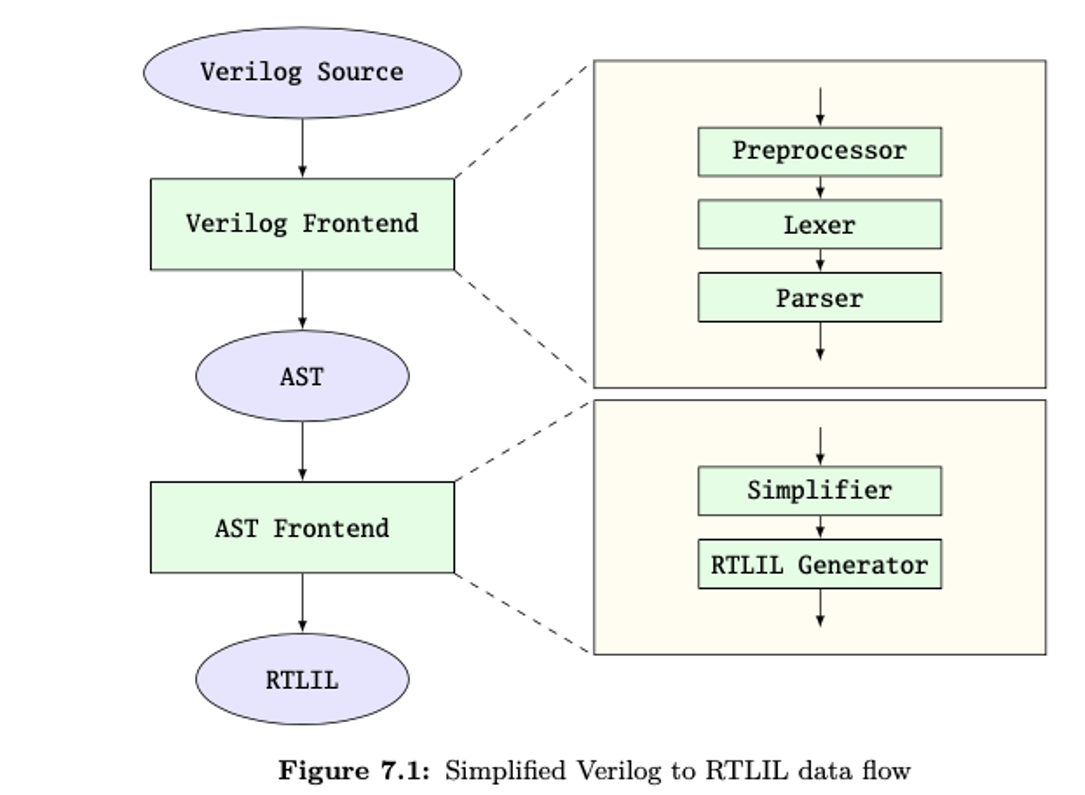
\includegraphics[scale=0.5]{verilogtortlil.png}
\end{center}

Das Inputstreamobjekt \textit{lexin} wird in verilog\_frontend.cc genutzt.

\begin{lstlisting}[language=C++]
if (!flag_nopp) {
code_after_preproc = frontend_verilog_preproc(*f, filename, defines_map, 
*design->verilog_defines, include_dirs);
	if (flag_ppdump)
		log("-- Verilog code after preprocessor
	 	--\n%s-- END OF DUMP --\n",code_after_preproc.c_str());
	lexin = new std::istringstream(code_after_preproc);
		}
\end{lstlisting} 

Das Streamobjekt \textit{f}, das dem Preprozessor übergeben wird, wird im Konstruktor der hierarchisch höheren Funktion übergeben:
\begin{lstlisting}[language=C++]
void execute(std::istream *&f, std::string filename,
std::vector<std::string> args, RTLIL::Design *design) override
\end{lstlisting}

\textit{code\_after\_preproc} ist also die Ausgabe des Preprozessors, deren Wert \textit{lexin} bekommt.

\textit{lexin} findet sich im Lexercode wieder:

\begin{lstlisting}[language=C++]
	#define YY_INPUT(buf,result,max_size) \
	result = readsome(*VERILOG_FRONTEND::lexin, buf, max_size)
\end{lstlisting}

Die Funktion \textit{readsome} ist folgende:
\begin{lstlisting}[language=C++]
int readsome(std::istream &f, char *s, int n)
{
	int rc = int(f.readsome(s, n));

	// f.readsome() sometimes returns 0 on a non-empty stream..
	if (rc == 0) {
		int c = f.get();
		if (c != EOF) {
			*s = c;
			rc = 1;
		}
	}

	return rc;
}
\end{lstlisting}

Es wird ein istream Objekt f, ein Char-Array *s und ein Integer n übergeben.
Aus f wird mit readsome eine Anzahl n Zeichen in ein Char-Array s geladen. Die Rückgabe ist die Anzahl an Zeichen, die geladen wurden. Danach kommt eine Behandlung für den Fall, dass rc == 0, wobei es sein kann, dass das istream Objekt nicht wirklich leer ist.\\
\\
In der Funktion YY\_INPUT wird also der Inputstream \textit{lexin} in den Buffer \textit{buf} geladen, bis \textit{max\_size} erreicht ist.
In result steht später eine 1, wenn ein Lesevorgang erfolgreich war. 

Im \textit{Flex} Manual steht zu YY\_INPUT, dass, wenn diese Funktion auf einen Eingang definiert ist (hier \textit{lexin}), der Funktionsaufruf des Lexers mit einem Nullpointer als Argument durchgeführt werden kann.



Später erfolgen folgende Funktionsaufrufe:
\begin{lstlisting}[language=C++]
		frontend_verilog_yyset_lineno(1);
		frontend_verilog_yyrestart(NULL);
		frontend_verilog_yyparse();
		frontend_verilog_yylex_destroy();
\end{lstlisting}

Die Funktion \textit{frontend\_verilog\_yyrestart} wird mit einem Nullpointer wie vorher diskutiert aufgerufen. Damit wird \textit{Flex} also mit der Eingabe lexin aufgerufen.\\
Normalerweise ist die \textit{Flex} Hauptfunktion \textit{yylex()}.
Hier wird \textit{yyrestart()} benutzt. Dies könnte damit zusammen hängen, dass ein Inputstream eingestellt wird. Außerdem bleiben bei \textit{yyrestart()} die Anfangsbedingungen der Regeln erhalten.\\
\\
Mit yyparse() wird dann der Parser aufgerufen. In dem Parserquellcode wird \textit{yylex()} aufgerufen. Die Integer Rückgabe wird in yychar gespeichert. Danach wird die Funktion \textit{yytranslate()} auf yychar aufgerufen, die eine zu dem Integer korrespondierende Symbolnummer zurückgibt. Diese wird in \textit{yytoken} gespeichert. Diese Variable ist vom Typ \textit{yysymbol\_kind\_t}.
\\
\\
In dem Parserquellcode existiert eine lange Case-Anweisung für die Integer Variable \textit{yyn}. Hier wird die AST-Struktur gebaut. \textit{yyn} wird an einer Stelle mit \textit{yytoken} inkrementiert.





\chapter{Parser}

Der Parser wird wie der Lexer automatisiert anhand einer Grammatikdatei .y gebaut. Hier wird anstatt \textit{Flex} der Open-Source Parsergenerator \textit{Bison} genutzt.
\section{Analyse des Parser-Quellcodes}
Die Parsergrammatik ist ähnlich wie die \textit{Flex} Beschreibung aufgebaut:
\begin{lstlisting}[language=C++]
%{
C declarations
%}
Bison declarations

%%
Grammar rules
%%

Additional C code
\end{lstlisting}

Im folgenden werden die Grammatikregeln analysiert:
\subsection{Analyse der Parser-Grammatik}
Um die Grammatikregeln zu verstehen, ist es notwendig, deren Zusammensetzung nachzuvollziehen.

Eine Grammatikregel in der Backus-Naur Form sieht so aus:

\begin{lstlisting}[language=C++]
result: components...
        ;
\end{lstlisting}
Result ist ein Nicht-Terminalsymbol. Component sind Terminal- und Nicht-Terminalsymbole.\\
Terminalsymbole sind Symbole, die einzeln nicht weiter durch Produktionsregeln ersetzt werden können.
Eine Beispielregel wäre folgende:

  \begin{lstlisting}[language=C++]
  	exp:      exp '+' exp
        ;

  \end{lstlisting}

exp '+' exp kann also in einer Produktion mit exp ersetzt werden.
\\
\\
Es folgt ein Beispiel für einen Taschenrechner, der mit Klammern Addieren und Multiplizieren kann.
Zuerst wird ein Lexer mit \textit{Flex} gebaut, der die Eingabe in Tokens zerlegt.
\begin{lstlisting}[language=C++]
%{
#include <stdio.h>
#include <string.h>
#include "add.tab.h"



%}

%option noyywrap

%%

[0-9]+  { yylval.zahl = atoi(yytext); return(ZAHL);}
"+" {return(PLUS);}
"=" {return(GLEICH);}
";" {return(SEMIKOLON);}
"*" {return(MAL);}
"(" {return(KLOFFEN);}
")" {return(KLZU);}
"\n" {return(RETURN);}
.   {return(OTHER);}



%%
\end{lstlisting}

Hier ist es wichtig, dass der Lexer in seiner \textit{Declaration} Sektion den Header des zukünftigen Bison Parsers übergeben bekommt. Die Header-Datei wird Standardmäßig immer so bezeichnet: "nameder.ydatei".tab.h. In dieser Headerdatei stehen die Integerwerte für die Tokenrückgabe für die Interpretation des Parsers.\\
\\
Es folgt die Parser Grammatik:

\begin{lstlisting}[language=C++]
	
%{

#include <stdio.h>

extern int yylex();
extern int yyparse();
int yyerror(char *s);


%}

//alle Tokens
%token ZAHL PLUS GLEICH SEMIKOLON OTHER MAL RETURN KLOFFEN KLZU

//ZAHL bekommt einen Wert vom Typ zahl
%type <zahl> ZAHL
%type <zahl> faktor
%type <zahl> term
%type <zahl> ausdruck


//Definition des Typs zahl
%union{
    int zahl;
}

%%

prog:
    ausdruck {
            printf("Ergebnis: %d", $1);
        }
;
ausdruck:
    ausdruck PLUS ausdruck{
        $$=$1+$3;
    }
    | term{
        $$=$1;
    }
;
term:
    term MAL term{
            $$=$1*$3;
    }
    | faktor{
            $$=$1;
    }
;
faktor:
    KLOFFEN ausdruck KLZU{
        $$=$2;
    }
    | ZAHL{
        $$=$1;
    }
;

%%

int yyerror(char *s)
{
	printf("Syntax Fehler in Zeile %s\n", s);
	return 0;
}

int main()
{
    yyparse();
    return 0;
}
\end{lstlisting}

In der Declarationssektion wird dem Parser übergeben, dass es eine yylex(), eine yyparse() und eine yyerror() Funktion gibt.
Danach werden in der \textit{Definitions} alle Tokens aufgelistet, die von dem Lexer übergeben werden können.\\
In dieser Sektion werden außerdem die Datentypen aller wertbehafteten Tokens sowie der im Parser definierten Nichtterminalsymbole mit \%type definiert. In \%union werden die Parser-Datentypen mit C-Datentypen verknüpft.\\
Anschließend folgen die Grammatik-Regeln.
\begin{center}
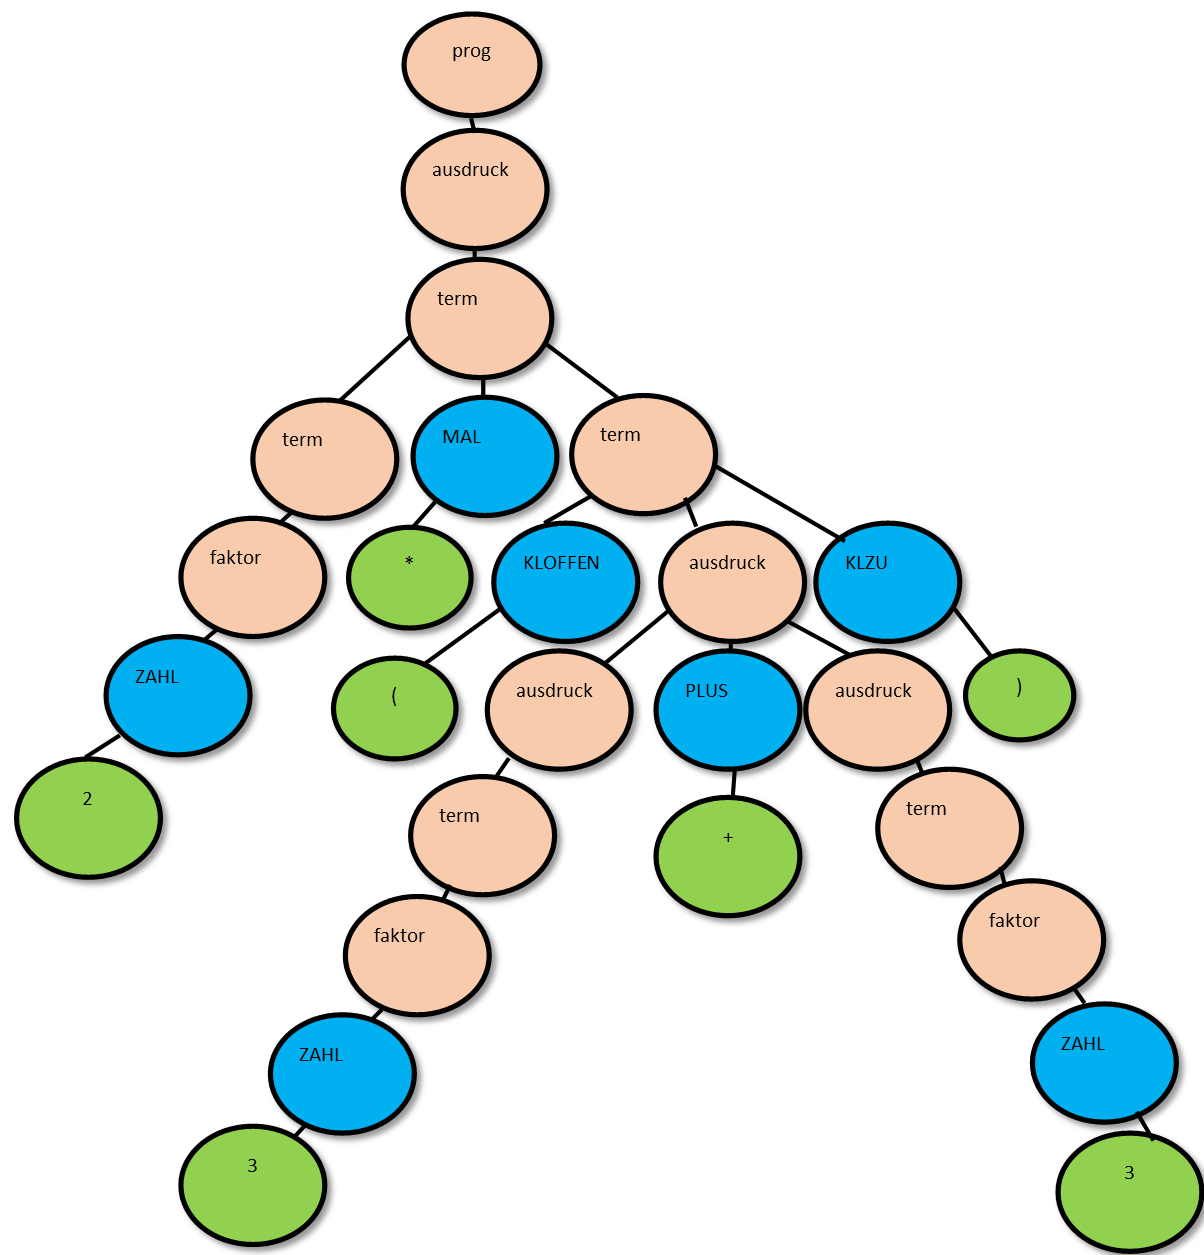
\includegraphics[scale=0.6]{Publikation1.png}
\\
\textit{Parserbaum für die Eingabe 2*(3+3). Zeichen sind grün, Tokens blau und die definierten Nichtterminalsymbole orange dargestellt.}
\end{center}

%TODO Tutorial mit Kompilierung

Dieses Verständnis wird nun auf den Verilogparser übertragen. Aufgrund des großen Umfangs der Grammatik, dessen Ableitungen nicht so einfach analysiert werden können, wie die Tokengeneration im Lexer, wird die Parsergrammatik anhand eines Beispiels analysiert.\\
\\
Die Analyse findet anhand des Verilog Ausdrucks \textit{assign} statt.
Ein einfaches Beispielmodul wäre folgendes:
\begin{lstlisting}[language=C++]
	module behave;
		wire i1,i2;
		wire out;
		assign out = i1 & i2;
	endmodule
\end{lstlisting}
\begin{enumerate}
  \item Vom Lexer wird für \textit{assign} der Token TOK\_ASSIGN zurückgegeben.
  \item Im Parser steht folgende Grammatikregel:
  \begin{lstlisting}[language=C++]
  assign_stmt:
  	TOK_ASSIGN delay assign_expr_list ';';
  \end{lstlisting}
  Für delay gibt es folgende Regel:
  \begin{lstlisting}[language=C++]
  	delay:
	non_opt_delay | %empty;
  \end{lstlisting}
  delay kann also auch ein leeres Zeichen sein, was zu dem Beispiel passt.
  Zusätzlich dazu kommt non\_opt\_delay:
  \begin{lstlisting}[language=C++]
  	non_opt_delay:
	'#' TOK_ID { delete $2; } |
	'#' TOK_CONSTVAL { delete $2; } |
	'#' TOK_REALVAL { delete $2; } |
	'#' '(' mintypmax_expr ')' |
	'#' '(' mintypmax_expr ',' mintypmax_expr ')' |
	'#' '(' mintypmax_expr ',' mintypmax_expr ',' mintypmax_expr ')';
  \end{lstlisting}
  Da nicht weiter auf den Wert der Eingabe reagiert wird, kann interpretiert werden, dass dies eine Inkompatibilität von Yosys ist, die ignoriert wird.\\
  Interessant wird hier assign\_expr\_list:
  \begin{lstlisting}[language=C++]
  	assign_expr_list:
	assign_expr | assign_expr_list ',' assign_expr;
  \end{lstlisting}
  Mit folgender Erweiterung:
  \begin{lstlisting}[language=C++]
  	assign_expr:
	lvalue '=' expr {
		AstNode *node = new AstNode(AST_ASSIGN, $1, $3);
		SET_AST_NODE_LOC(node, @$, @$);
		ast_stack.back()->children.push_back(node);
	};
  \end{lstlisting}
  Hier lässt sich die konkrete Zuweisung erkennen. 
  Als Reaktion wird eine AstNode mit dem Typ AST\_ASSIGN erstellt, dessen Children die Werte von lvalue und expr bekommen.
  Für die weitere Auswertung ist eine weitere Erweiterung möglich:
  \begin{lstlisting}[language=C++]
  	expr:
	basic_expr {
		$$ = $1;
	} |
	basic_expr '?' attr expr ':' expr {
		$$ = new AstNode(AST_TERNARY);
		$$->children.push_back($1);
		$$->children.push_back($4);
		$$->children.push_back($6);
		SET_AST_NODE_LOC($$, @1, @$);
		append_attr($$, $3);
	};
  \end{lstlisting}
Mit basic\_expr: (Ausschnitt wegen langer Anweisung)
\begin{lstlisting}[language=C++]
	} |
	basic_expr OP_LAND attr basic_expr {
		$$ = new AstNode(AST_LOGIC_AND, $1, $4);
		SET_AST_NODE_LOC($$, @1, @4);
		append_attr($$, $3);
	} |
	basic_expr OP_LOR attr basic_expr {
		$$ = new AstNode(AST_LOGIC_OR, $1, $4);
		SET_AST_NODE_LOC($$, @1, @4);
		append_attr($$, $3);
	} |
	'!' attr basic_expr %prec UNARY_OPS {
		$$ = new AstNode(AST_LOGIC_NOT, $3);
		SET_AST_NODE_LOC($$, @1, @3);
		append_attr($$, $2);
	} |
\end{lstlisting}

expr besteht also aus allen möglichen logischen Verknüpfungen, mathematischen Funktionen und Vergleichen.
\item assign\_stmt kann weiter reduziert werden:
\begin{lstlisting}[language=C++]
	module_body_stmt:
	task_func_decl | specify_block | param_decl | localparam_decl
	| typedef_decl | defparam_decl | specparam_declaration | wire_decl 
	| assign_stmt | cell_stmt 
	| enum_decl | struct_decl 
	| always_stmt | TOK_GENERATE module_gen_body TOK_ENDGENERATE
	| defattr | assert_property | checker_decl
	| ignored_specify_block;
\end{lstlisting}
ODER:
\begin{lstlisting}[language=C++]
	interface_body_stmt:
	param_decl | localparam_decl | typedef_decl 
	| defparam_decl | wire_decl | always_stmt | assign_stmt |
	modport_stmt;
\end{lstlisting}

Hier sind zwei also zwei Reduktionen möglich! Dies führt zu einem Konflikt. Bison meldet in einem mehrdeutigen Fall wie diesem eine \textbf{reduce/reduce conflict} Warnung.
\item Für module\_body\_stmt ist folgende Reduktion möglich:
\begin{lstlisting}[language=C++]
	module_body:
	module_body module_body_stmt |
	/* the following line makes the generate..
	endgenrate keywords optional */
	module_body gen_stmt |
	module_body gen_block |
	module_body ';' |
	%empty;
\end{lstlisting}

Für interface\_body\_stmt:
\begin{lstlisting}[language=C++]
	interface_body:
	interface_body interface_body_stmt | %empty;
\end{lstlisting}

Auffällig ist, dass diese Reduzierungen jeweils nur eine weitere Stufe ohne weitere Reaktionen / Verknüpfungen sind.
\item
module\_body wird zu module reduziert:
\begin{lstlisting}[language=C++]
	module:
	attr TOK_MODULE {
		enterTypeScope();
	} TOK_ID {
		do_not_require_port_stubs = false;
		AstNode *mod = new AstNode(AST_MODULE);
		ast_stack.back()->children.push_back(mod);
		ast_stack.push_back(mod);
		current_ast_mod = mod;
		port_stubs.clear();
		port_counter = 0;
		mod->str = *$4;
		append_attr(mod, $1);
		delete $4;
	} module_para_opt module_args_opt ';' module_body 
	TOK_ENDMODULE opt_label {
		if (port_stubs.size() != 0)
			frontend_verilog_yyerror(
			"Missing details for module port `%s'.",
				port_stubs.begin()->first.c_str());
		SET_AST_NODE_LOC(ast_stack.back(), @2, @$);
		ast_stack.pop_back();
		log_assert(ast_stack.size() == 1);
		current_ast_mod = NULL;
		exitTypeScope();
	};
\end{lstlisting}

\item
module wird auf design reduziert. Hier ist sichtbar, dass ein design durch den Wiederaufruf aus mehren Modulen oder anderen Bestandteilen entstehen kann.

\begin{lstlisting}[language=C++]
	design:
	module design |
	defattr design |
	task_func_decl design |
	param_decl design |
	localparam_decl design |
	typedef_decl design |
	package design |
	interface design |
	%empty;
\end{lstlisting}

\item
Zuletzt wird design auf inout reduziert.
\begin{lstlisting}[language=C++]
	input: {
	ast_stack.clear();
	ast_stack.push_back(current_ast);
} design {
	ast_stack.pop_back();
	log_assert(GetSize(ast_stack) == 0);
	for (auto &it : default_attr_list)
		delete it.second;
	default_attr_list.clear();
};
\end{lstlisting}

\end{enumerate}

In einigen der Reduktionen wird mit AST-Strukturen gearbeitet.
AST-Stack ist eine Datenstruktur vom Typ Vector:
\begin{lstlisting}[language=C++]
	std::vector<AstNode*> ast_stack;
\end{lstlisting}
Vektoren sind sequentielle Datenstrukturen wie Arrays, jedoch mit dynamischer Länge.
Die Vektorstruktur wird hier genutzt, um einen Stack zu repräsentieren.
\\
\\
Ein Stack ist eine LIFO-Struktur, die als C-Vektor nach unten wächst. Das letzte Element was auf den Stack gelegt wird (push\_back(objekt)) wird als erstes ausgegeben (back()). Es ist üblich, das erste Stackobjekt nach dem lesen zu entfernen (pop\_back()).
\\
\\
Die Objekte, die auf diesen Stack gelegt werden, sind vom Typ AstNode und repräsentieren die Knoten des Abstrakten-Syntax-Baums.
Hier ist ein Ausschnitt der Struktur.
\begin{lstlisting}[language=C++]
	struct AstNode
	{
		// for dict<> and pool<>
		unsigned int hashidx_;
		unsigned int hash() const { return hashidx_; }

		// this nodes type
		AstNodeType type;

		// the list of child nodes for this node
		std::vector<AstNode*> children;

		// the list of attributes assigned to this node
		std::map<RTLIL::IdString, AstNode*> attributes;
		bool get_bool_attribute(RTLIL::IdString id);

		// node content - most of it is unused in most node types
		std::string str;
		std::vector<RTLIL::State> bits;
		bool is_input, is_output, is_reg, is_logic, is_signed, 
		is_string, is_wand, is_wor, range_valid, range_swapped, 
		was_checked, is_unsized, is_custom_type;
		int port_id, range_left, range_right;
		uint32_t integer;
		double realvalue;
		// set for IDs typed to an enumeration, not used
		bool is_enum;
\end{lstlisting}
Gespeichert sind also Eigenschaften wie beispielsweise Typ, children (hierarchisch niedrigere Knoten im Baum), Attribute und Inhalt.
\\
\\

\begin{lstlisting}[language=C++]
	AstNode *mod = new AstNode(AST_MODULE);
		ast_stack.back()->children.push_back(mod);
		ast_stack.push_back(mod);
\end{lstlisting}

In der module-Regel wird ein neuer Knoten AST\_MODULE erstellt. Das letzte Stackobjekt bekommt diesen Knoten als Children angehangen. Danach wird der Knoten selbst auf den Stack gelegt. ast\_stack und children sind also separate Stacks. Jede Node hat einen stack children, wie bereits zuvor in der AST-Struktur zu sehen war.
\begin{lstlisting}[language=C++]
	current_ast_mod = mod;
		port_stubs.clear();
		port_counter = 0;
		mod->str = *$4;
		append_attr(mod, $1);
		delete $4;
\end{lstlisting}


Im Yosys Manual wird folgender Parserbaum für ein assign Statement dargestellt:
\begin{center}
	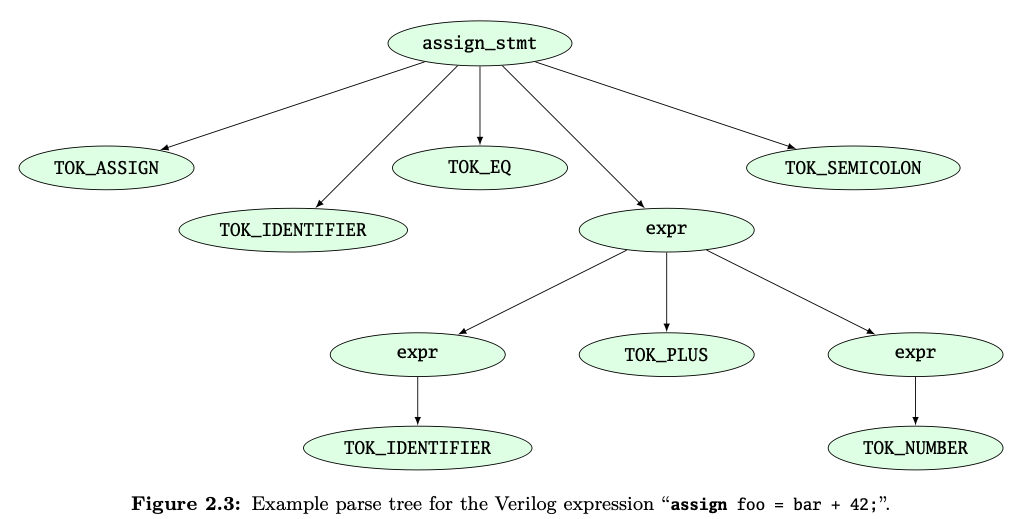
\includegraphics[scale=0.4]{assignstmt.png}
\end{center}

Bei Betrachtung der Reduzierungen unter Beachtung der Parserregeln fällt jedoch auf, dass diese Grafik nicht mehr aktuell sein kann.
Es sind einige Reduktionen notwendig, die hier nicht berücksichtigt werden. Ein Problem dabei sind Konflikte, da teilweise verschiedene Reduktionen möglich sind.

\subsection{Interpretations-Probleme}
\begin{enumerate}
  \item Reduzierungskonflikte
\\
\\
Wie priorisiert der Parser Regeln. Woher kommt der Determinismus? Welche Rolle spielen der Parsertyp LALR (Look-Ahead-Left-Right) und die Bison precendence Regeln?
  \item Stackaufbau
\\
\\
Wie wird der Masterstack ast\_stack aufgebaut? Wann werden Objekte auf den Stapel gelegt? 
\end{enumerate}

Unter Vernachlässigung dieser Probleme wird die Parseranalyse an dieser Stelle beendet und es wird davon ausgegangen, dass AST-Stack Strukturen gebildet wurden.
\\
\\
Diese Strukturen werden von dem AST-Frontend weiterverarbeitet.
\chapter{AST-Frontend}
Das AST-Frontend überführt die AST-Strukturen in die interne Registertransfer-Level Sprache RTLIL.
Laut Yosys-Manual findet die Überführung in RTLIL in zwei Schritten statt:
\begin{enumerate}
  \item Vereinfachung (Simplification)
  \item RTLIL Generation
\end{enumerate}

In der Struktur AstNode in der Headerdatei ast.h ist eine Funktion für die Vereinfachung deklariert:
\begin{lstlisting}[language=C++]
	bool simplify(bool const_fold, bool at_zero, 
	bool in_lvalue, int stage, int width_hint, 
	bool sign_hint, bool in_param);
\end{lstlisting}

Laut Manual werden folgende Vereinfachungen durchgeführt:

\begin{enumerate}
  
\item Inline all task and function calls.
\item Evaluate all generate-statements and unroll all for-loops.
\\
\\
Generate-Blöcke erzeugen mehrere Instanzen eines Moduls oder ermöglichen die bedingte Instanziierung eines Moduls. Hier werden also alle Instanzen evaluiert. \\
For-Schleifen werden abgewickelt, indem die Iterationsanzahl verringert wird



\item Perform const folding where it is necessary (e.g. in the value part of AST\_PARAMETER, AST\_LOCALPARAM, AST\_PARASET and AST\_RANGE nodes).
\\
\\
Folding (oder auch Falten) ist ein Prozess, bei dem die Anzahl von funktionalen Blöcken reduziert wird, indem Register und Multiplexer eingesetzt werden.

\item Replace AST\_PRIMITIVE nodes with appropriate AST\_ASSIGN nodes.
\\
\\
Verilog Primitives sind von folgender Form:
\begin{lstlisting}[language=C++]
	and (out, in1, in2, in3);
\end{lstlisting}
Diese Form entspricht nicht den gewöhnlichen assign-Statements, kann jedoch einfach umgewandelt werden. Dies vereinfacht die Konvertierung nach RTLIL, da die Primitives mit assign-Statements abgedeckt werden. 


\item Replace dynamic bit ranges in the left-hand-side of assignments with AST\_CASE nodes with AST\_COND
children for each possible case.
\\
\\
Dynamische Wortgrößen müssen deterministisch festgelegt werden.
Dafür werden AST\_CASE nodes für die Fallunterscheidung eingesetzt. Die children dieser Nodes sind die Fälle.

\item Detect array access patterns that are too complicated for the RTLIL::Memory abstraction and replace them with a set of signals and cases for all reads and/or writes.
\\
\\
Komplizierte Speicherzugriffsmuster werden mit Signalen und Fällen für alle Lese- und Schreibzugriffe ersetzt.
\item Otherwise replace array accesses with AST\_MEMRD and AST\_MEMWR nodes.
\\
\\
Standardbehandlung für Lese- und Schreibzugriffe auf Speicher ist mit AST\_MEMRD und AST\_MEMWR Nodes.

\end{enumerate}

\section{Analyse der simplify Funktion}

Die simplify-Funktion ist in der Datei simplify.cc enthalten.

\begin{lstlisting}[language=C++]
		static int recursion_counter = 0;
	static bool deep_recursion_warning = false;

	if (recursion_counter++ == 1000 && deep_recursion_warning) {
		log_warning("Deep recursion in AST simplifier.\n
		Does this design contain insanely long expressions?\n");
		deep_recursion_warning = false;
	}

	AstNode *newNode = NULL;
	bool did_something = false;
\end{lstlisting}

Der Anfang der Funktion beinhaltet einen recursion counter, der bei Aufruf der Bedingung inkrementiert wird. Die Vereinfachungen scheinen also rekursiv aufgerufen zu werden. Ab 1000 Aufrufen zählt dies hier als \textit{deep recursion} (tiefe Rekursion).
\\
\\
Es werden die angesprochenen Vereinfachungen im Quellcode gesucht.

\begin{lstlisting}[language=C++]
// unroll for loops and generate-for blocks
	if ((type == AST_GENFOR || type == AST_FOR) && children.size() != 0)
	{
		AstNode *init_ast = children[0];
		AstNode *while_ast = children[1];
		AstNode *next_ast = children[2];
		AstNode *body_ast = children[3];

		while (body_ast->type == AST_GENBLOCK && 
		body_ast->str.empty() &&
		body_ast->children.size() == 1 && 
		body_ast->children.at(0)->type == AST_GENBLOCK)
		body_ast = body_ast->children.at(0);
\end{lstlisting}

Ein generate-for Block generiert Instanzen eines Moduls bei jedem Aufruf der for-Schleife.\\
\\
Die Reihenfolge der children jeder AST-Node scheint eine große Bedeutung zu haben, da diese Nodes in Kategorien eingeteilt werden.
\\
\\
Das Ausrollen geschieht durch das Auswerten von drei Ausdrücken.
\begin{lstlisting}[language=C++]
	// eval 1st expression
	AstNode *varbuf = init_ast->children[1]->clone();
	{
	int expr_width_hint = -1;
	bool expr_sign_hint = true;
	varbuf->detectSignWidth(expr_width_hint, expr_sign_hint);
	while (varbuf->
	simplify(true, false, false, stage, 32, true, false)) { }
		}

if (varbuf->type != AST_CONSTANT)
	log_file_error(filename, linenum, "Right hand side of 
	1st expression of generate for-loop is not constant!\n");

	varbuf = new AstNode(AST_LOCALPARAM, varbuf);
	varbuf->str = init_ast->children[0]->str;

	AstNode *backup_scope_varbuf = current_scope[varbuf->str];
	current_scope[varbuf->str] = varbuf;

	size_t current_block_idx = 0;
	if (type == AST_FOR) {
	while (current_block_idx < current_block->children.size() &&
		current_block->
		children[current_block_idx] != current_block_child)
		current_block_idx++;
		}
\end{lstlisting}

Die Breite oder hier \textit{Width} eines Signals ist Teil der Range.



\section{Analyse der genRTLIL Funktion}

genRTLIL ist Teil der Strukturdefinition für Syntaxbaum-Knoten AstNode. 
\\
\\
Die genRTLIL Funktion besteht zu einem Teil aus einer großen Case-Bedingung.

\begin{lstlisting}[language=C++]
	switch (type)
	{
	// simply ignore this nodes.
	// they are either leftovers from simplify() or
	 are referenced by other nodes
	// and are only accessed here thru this references
	case AST_NONE:
	case AST_TASK:
	case AST_FUNCTION:
	case AST_DPI_FUNCTION:
	case AST_AUTOWIRE:
	case AST_DEFPARAM:
	case AST_GENVAR:
	case AST_GENFOR:
	case AST_GENBLOCK:
	case AST_GENIF:
	case AST_GENCASE:
	case AST_PACKAGE:
	case AST_MODPORT:
	case AST_MODPORTMEMBER:
		break;
\end{lstlisting}

Diese Blöcke werden ignoriert, da sie Überbleibsel der simplify-Funktion sind oder mit anderen Knoten behandelt werden. Hier ist auffällig, dass unteranderem die Generate-Blöcke enthalten sind, die in der simplify-Funktion ausgerollt werden.

\section{Prozessgenerator}

Der Prozessgenerator behandelt always-Blöcke.
Laut Yosys-Manual passiert zuerst folgendes:
\\
\\
\textit{
On startup the ProcessGenerator generates a new RTLIL::Process object with an empty root case and initializes its state variables as described above. Then the RTLIL::SyncRule objects are created using the synchronization events from the AST\_ALWAYS node and the initial values of subst\_lvalue\_from and subst\_lvalue\_to. Then the AST for this process is evaluated recursively.
}
\\
\\
Dies deckt sich mit dem Quellcode:
\begin{lstlisting}[language=C++]
RTLIL::CaseRule *current_case;
stackmap<RTLIL::SigBit, RTLIL::SigBit> subst_rvalue_map;
stackmap<RTLIL::SigBit, RTLIL::SigBit> subst_lvalue_map;
\end{lstlisting}
Später:
\begin{lstlisting}[language=C++]
// create syncs for the process
bool found_clocked_sync = false;
for (auto child : always->children)
	if (child->type == AST_POSEDGE || child->type == AST_NEGEDGE) {
		if (GetSize(child->children) == 1 && 
		 child->children.at(0)->type == 
		 AST_IDENTIFIER && child->children.at(0)->id2ast &&
		 child->children.at(0)->id2ast->type == AST_WIRE && 
		 child->children.at(0)->id2ast->get_bool_attribute("\\gclk"))
		continue;
	found_clocked_sync = true;
	if (found_global_syncs || found_anyedge_syncs)
	 log_file_error(always->filename, always->linenum, 
	 "Found non-synthesizable event list!\n");
	RTLIL::SyncRule *syncrule = new RTLIL::SyncRule;
	syncrule->type = child->type == AST_POSEDGE ? RTLIL::STp : RTLIL::STn;
	syncrule->signal = child->children[0]->genRTLIL();
	if (GetSize(syncrule->signal) != 1)
	 log_file_error(always->filename, always->linenum, 
	 "Found posedge negedge event on a signal that is not 1 bit wide!\n");
	addChunkActions(syncrule->actions, subst_lvalue_from, 
	subst_lvalue_to,true);
	proc->syncs.push_back(syncrule);
			}
\end{lstlisting}
%Strukturen
\subsection{Strukturen}
\begin{enumerate}
  \item \textit{lvalue}
\\
Bekommt Rückgabe der genRTLIL() Funktion zugewiesen. Rückgabetyp ist RTLIL::SigSpec
\item \textit{SigSpec}
Aus dem Manual:
\textit{The RTLIL::SigSpec data type is used to represent signals. The RTLIL::Cell object contains one RTLIL::SigSpec
for each cell port.
In addition, connections between wires are represented using a pair of RTLIL::SigSpec objects. Such pairs are needed in different locations. Therefore the type name RTLIL::SigSig was defined for such a pair.}
\begin{lstlisting}[language=C++]
struct RTLIL::SigSpec
{
private:
	int width_;
	unsigned long hash_;
	std::vector<RTLIL::SigChunk> chunks_; // LSB at index 0
	std::vector<RTLIL::SigBit> bits_; // LSB at index 0

	void pack() const;
	void unpack() const;
	void updhash() const;

	inline bool packed() const {
		return bits_.empty();
	}

	inline void inline_unpack() const {
		if (!chunks_.empty())
			unpack();
	}
\end{lstlisting}
...

SigSpec besitzt remove Funktionen, um ein Muster zu löschen. Das Muster kann aus einzelnen Signal-Bits SigBit, Signalen SigSpecs, die generell Vektoren aus Sigbits sind und Mischungen bestehen.

\begin{lstlisting}[language=C++]
	void replace(const RTLIL::SigSpec &pattern, const RTLIL::SigSpec &with);
	void replace(const RTLIL::SigSpec &pattern, const RTLIL::SigSpec &with, RTLIL::SigSpec *other) const;

	void replace(const dict<RTLIL::SigBit, RTLIL::SigBit> &rules);
	void replace(const dict<RTLIL::SigBit, RTLIL::SigBit> &rules, RTLIL::SigSpec *other) const;

	void replace(const std::map<RTLIL::SigBit, RTLIL::SigBit> &rules);
	void replace(const std::map<RTLIL::SigBit, RTLIL::SigBit> &rules, RTLIL::SigSpec *other) const;

	void replace(int offset, const RTLIL::SigSpec &with);

	void remove(const RTLIL::SigSpec &pattern);
	void remove(const RTLIL::SigSpec &pattern, RTLIL::SigSpec *other) const;
	void remove2(const RTLIL::SigSpec &pattern, RTLIL::SigSpec *other);

	void remove(const pool<RTLIL::SigBit> &pattern);
	void remove(const pool<RTLIL::SigBit> &pattern, RTLIL::SigSpec *other) const;
	void remove2(const pool<RTLIL::SigBit> &pattern, RTLIL::SigSpec *other);
	void remove2(const std::set<RTLIL::SigBit> &pattern, RTLIL::SigSpec *other);
\end{lstlisting}

\item Ersetzungsmuster in \textit{subst\_rvalue\_map} und \textit{subst\_lvalue\_map}.
\begin{lstlisting}[language=C++]
	// This map contains the replacement pattern to be used in the right hand side
	// of an assignment. E.g. in the code "foo = bar; foo = func(foo);" the foo in the right
	// hand side of the 2nd assignment needs to be replace with the temporary signal holding
	// the value assigned in the first assignment. So when the first assignment is processed
	// the according information is appended to subst_rvalue_from and subst_rvalue_to.
	stackmap<RTLIL::SigBit, RTLIL::SigBit> subst_rvalue_map;

	// This map contains the replacement pattern to be used in the left hand side
	// of an assignment. E.g. in the code "always @(posedge clk) foo <= bar" the signal bar
	// should not be connected to the signal foo. Instead it must be connected to the temporary
	// signal that is used as input for the register that drives the signal foo.
	stackmap<RTLIL::SigBit, RTLIL::SigBit> subst_lvalue_map;
\end{lstlisting}

Stackmaps (Yosys-Customs) sind ähnlich wie Maps in C++ mit der Erweiterung, dass Zustände gespeichert und wiederhergestellt werden können. Elemente können mit einem Schlüssel gespeichert werden und mit diesem Schlüssel wieder ausgelesen werden (vgl. Hashmap).

\item \textit{current\_state} \\
Ein konstantes Hashlib \textit{dict} Objekt. Ein Dictionary ist ähnlich wie eine  Hashmap. Es können jedoch nur Paare von gleichem Datentyp gespeichert werden. Ein Dictionary ist jedoch schneller und behält seine Ordnung.
\item \textit{current\_case}\\
\begin{lstlisting}[language=C++]
struct RTLIL::CaseRule : public RTLIL::AttrObject
{
	std::vector<RTLIL::SigSpec> compare;
	std::vector<RTLIL::SigSig> actions;
	std::vector<RTLIL::SwitchRule*> switches;

	~CaseRule();
	void optimize();

	bool empty() const;

	template<typename T> void rewrite_sigspecs(T &functor);
	template<typename T> void rewrite_sigspecs2(T &functor);
	RTLIL::CaseRule *clone() const;
};
\end{lstlisting}
Laut Manual der aktuelle Case der gerade gefüllt wird. Actions sind Zuweisungen. Ein Case kann außerdem weitere Switches besitzen.
\item \textit{SigSig}\\
Verbindungen von zwei Signalen werden als Paar aus zwei SigSpec Signalen SigSig implementiert:
\begin{lstlisting}[language=C++]
	typedef std::pair<SigSpec, SigSpec> SigSig;
\end{lstlisting}

\end{enumerate}



\subsection{Non-Blocking Assignments}

Die Behandlung von Non-Blocking Assignments wird im Yosys Manual beschrieben. Hier werden die entsprechenden Einträge mit dem Quellcode aus der genRTLIL.cc Datei verglichen:
\\
\\
\textit{
When an AST\_ASSIGN\_LE node is discovered, the following actions are performed by the ProcessGenerator:
}
\begin{enumerate}
  \item The left-hand-side is evaluated using AST::AstNode::genRTLIL() and mapped to a temporary signal name using subst\_lvalue\_from and subst\_lvalue\_to.
  \begin{lstlisting}[language=C++]
case AST_ASSIGN_LE:
{
RTLIL::SigSpec unmapped_lvalue = 
ast->children[0]->genRTLIL(), lvalue = unmapped_lvalue;
	
  \end{lstlisting}
Das nullte Objekt auf dem children Stack einer ASSIGN Node ist die linke Seite einer Zuweisung.
Nochmal zur Erinnerung: Der AstNode Struktur werden folgende Parameter übergeben:
\begin{lstlisting}[language=C++]
AstNode::AstNode(AstNodeType type, AstNode *child1, 
AstNode *child2, AstNode *child3)
\end{lstlisting}

Daraus wird der children-Stack befüllt:
\begin{lstlisting}[language=C++]
	if (child1)
		children.push_back(child1);
	if (child2)
		children.push_back(child2);
	if (child3)
		children.push_back(child3);
\end{lstlisting}
 
Im Parser werden die Werte der linken und rechten Seite der Zuweisung wie folgt übergeben:
\begin{lstlisting}[language=C++]
assign_expr:
lvalue '=' expr {
	ast_stack.back()->
	children.push_back(new AstNode(AST_ASSIGN, $1, $3));
	};	
\end{lstlisting}

Child1 bekommt den Wert von lvalue, Child2 den Wert von expr.

  \item \textit{The right-hand-side is evaluated using AST::AstNode::genRTLIL(). For this call, the values of subst\_rvalue\_from and subst\_rvalue\_to are used to map blocking-assigned signals correctly.}
\begin{lstlisting}[language=C++]
RTLIL::SigSpec rvalue = 
ast->children[1]->genWidthRTLIL(lvalue.size(), 
&subst_rvalue_map.stdmap());
\end{lstlisting}   
  
Da eine Zuweisung nur möglich ist, wenn der Ausdruck auf der rechten Seite die gleiche Wortbreite wie der Ausdruck auf der linken Seite hat, wird hier ein Wrapper der RTLIL Funktion verwendet, der mit einem Parameter für die Breite (Width) Rücksicht darauf nimmt. Als Parameter wird lvalue.size(), also die Breite der linken Seite übergeben.\\
\\
subst\_rvalue\_map ist eine stackmap:
\begin{lstlisting}[language=C++]
stackmap<RTLIL::SigBit, RTLIL::SigBit> subst_rvalue_map;
\end{lstlisting}

Stackmap ist ein eigener Datentyp, der wie eine map funktioniert wobei zusätzlich der aktuelle Zustand gespeichert und wiederhergestellt werden kann.

  
  \item \textit{Remove all assignments to the same left-hand-side as this assignment from the current\_case and all
cases within it.}
\\
\\
Alle vorherigen Zuweisungen werden bei einem Non-Blocking Assignment überschrieben.

\begin{lstlisting}[language=C++]
	pool<SigBit> lvalue_sigbits;
	for (int i = 0; i < GetSize(lvalue); i++) {
		if (lvalue_sigbits.count(lvalue[i]) > 0) {
			unmapped_lvalue.remove(i);
			lvalue.remove(i);
			rvalue.remove(i--);
		} else
			lvalue_sigbits.insert(lvalue[i]);
				}
\end{lstlisting}

lvalue ist ein SigSpec Objekt.
Die SigSpec Struktur beschreibt ein Signal und hat einige Funktionen zur Manipulation.
Auszug:
\begin{lstlisting}[language=C++]
struct RTLIL::SigSpec
{
private:
	int width_;
	unsigned long hash_;
	std::vector<RTLIL::SigChunk> chunks_; // LSB at index 0
	std::vector<RTLIL::SigBit> bits_; // LSB at index 0
\end{lstlisting}

Die Zuweisung wird entfernt, indem durch eine Iteration durch das Signal mit remove(i) die Bits gelöscht werden:
\begin{lstlisting}[language=C++]
void RTLIL::SigSpec::remove(int offset, int length)
{
	cover("kernel.rtlil.sigspec.remove_pos");

	unpack();

	log_assert(offset >= 0);
	log_assert(length >= 0);
	log_assert(offset + length <= width_);

	bits_.erase(bits_.begin() + offset, 
	bits_.begin() + offset + length);
	width_ = bits_.size();

	check();
}
\end{lstlisting}

Das Iterationsobjekt i der for-Schleife ist also hier der Offset vom LSB.


\item \textit{Add the new assignment to the current\_case.
}
\begin{lstlisting}[language=C++]
lvalue.replace(subst_lvalue_map.stdmap());

if (ast->type == AST_ASSIGN_EQ) {
	for (int i = 0; i < GetSize(unmapped_lvalue); i++)
	subst_rvalue_map.set(unmapped_lvalue[i], rvalue[i]);
}
removeSignalFromCaseTree(lvalue, current_case);
remove_unwanted_lvalue_bits(lvalue, rvalue);
current_case->actions.push_back(RTLIL::SigSig(lvalue, rvalue));
\end{lstlisting}

Die replace() Funktion:
\begin{lstlisting}[language=C++]
void RTLIL::SigSpec::replace(const dict<RTLIL::SigBit, 
RTLIL::SigBit> &rules, RTLIL::SigSpec *other) const
{
	cover("kernel.rtlil.sigspec.replace_dict");

	log_assert(other != NULL);
	log_assert(width_ == other->width_);

	unpack();
	other->unpack();

	for (int i = 0; i < GetSize(bits_); i++) {
		auto it = rules.find(bits_[i]);
		if (it != rules.end())
			other->bits_[i] = it->second;
	}

	other->check();
}
\end{lstlisting}

rules ist in dem Fall subst\_lvalue\_map.stdmap(), also die Map mit temporären Signalen und other ist lvalue.

unpack() legt die Bits eines Signals auf einen Vektorstapel bits\_. Der Vektor kann auch stellenweise ausgelesen werden, was hier im weiteren Verlauf benutzt wird.
\\
\\
find() ist Teil der Hashlib und gibt einen Iterator zurück. Hier wird anscheinend ein dynamisches Objekt \textit{it} erzeugt, das den Wert von bits\_[i] bekommt.
Am Ende der for-Schleife werden werden die Bitvektorwerte bits\_[i] von other auf das zweite Paar-Objekt von it gesetzt.\\
(\url{https://stackoverflow.com/questions/15451287/what-does-iterator-second-mean})

\end{enumerate}


\subsection{Blocking-Assignments}


\textit{When an AST\_ASSIGN\_EQ node is discovered, the following actions are performed by the ProcessGenerator:}
\begin{enumerate}
  \item \textit{Perform all the steps that would be performed for a nonblocking assignment (see above).}
  \begin{lstlisting}[language=C++]
 case AST_ASSIGN_EQ:
 case AST_ASSIGN_LE:		
  \end{lstlisting}
  Da kein break; Abbruch der case-Bedingung erfolgt, geht das Programm in den nachfolgenden Case-Fall, der das Non-Blocking-Assignment behandelt.
\item \textit{Remove the found left-hand-side (before lvalue mapping) from subst\_rvalue\_from and also remove the respective bits from subst\_rvalue\_to.}



\item \textit{Append the found left-hand-side (before lvalue mapping) to subst\_rvalue\_from and append the found right-hand-side to subst\_rvalue\_to.}
\\
\\
In dem AST\_ASSIGN\_LE Case ist eine if-Bedingung für die Behandlung des Blocking Assignments.

\begin{lstlisting}[language=C++]
if (ast->type == AST_ASSIGN_EQ) {
					for (int i = 0; i < GetSize(unmapped_lvalue); i++)
						subst_rvalue_map.set(unmapped_lvalue[i], rvalue[i]);
				}
\end{lstlisting}

Bevor temporäre Signale gelöscht werden, wie es bei einem Non-Blocking Assignment der Fall ist, werden diese zwischengespeichert.

\end{enumerate}

\subsection{Cases und if-Anweisungen}

\textit{When an AST\_CASE node is discovered, the following actions are performed by the ProcessGenerator:}
\begin{enumerate}
  \item \textit{The values of subst\_rvalue\_from, subst\_rvalue\_to, subst\_lvalue\_from and subst\_lvalue\_to are pushed to the stack.}

  
\item \textit{A new RTLIL::SwitchRule object is generated, the selection expression is evaluated using AST::AstNode::genRTLIL() (with the use of subst\_rvalue\_from and subst\_rvalue\_to) and added to the RTLIL::SwitchRule object and the object is added to the current\_case.}
  \begin{lstlisting}[language=C++]
  	case AST_CASE:
			{
				RTLIL::SwitchRule *sw = new RTLIL::SwitchRule;
				sw->attributes["\\src"] = stringf("%s:%d", ast->filename.c_str(), ast->linenum);
				sw->signal = ast->children[0]->genWidthRTLIL(-1, &subst_rvalue_map.stdmap());
				current_case->switches.push_back(sw);
  \end{lstlisting}
  Ein SwitchRule Objekt sw wird erstellt.
  Die SwitchRule Struktur sieht so aus:
  \begin{lstlisting}[language=C++]
  	struct RTLIL::SwitchRule : public RTLIL::AttrObject
{
	RTLIL::SigSpec signal;
	std::vector<RTLIL::CaseRule*> cases;

	~SwitchRule();

	bool empty() const;

	template<typename T> void rewrite_sigspecs(T &functor);
	template<typename T> void rewrite_sigspecs2(T &functor);
	RTLIL::SwitchRule *clone() const;
};
  \end{lstlisting}
  Die SwitchRule Struktur besitzt also ein Signal und einen Vektor (Stapel) cases.
  Das Signal bekommt den RTLIL Code von subst\_rvalue\_map.stdmap(), die Ersetzung für Blocking-Assignments.

\item \textit{All lvalues assigned to within the AST\_CASE node using blocking assignments are collected and saved in the local variable this\_case\_eq\_lvalue.}
\begin{lstlisting}[language=C++]
RTLIL::SigSpec this_case_eq_lvalue;
				collect_lvalues(this_case_eq_lvalue, ast, true, false);
\end{lstlisting}
Erinnerung: AST\_ASSIGN\_EQ sind AstNodes für Blocking-Assignments.
Der Funktion collect\_lvalues hat Parameter für Blocking- und Non-Blocking Assignments:
\begin{lstlisting}[language=C++]
void collect_lvalues(RTLIL::SigSpec &reg, AstNode *ast, bool type_eq, bool type_le, bool run_sort_and_unify = true)
\end{lstlisting}
Über den Boolean \textit{type\_eq} kann also übergeben werden, dass nur lvalues von Blocking-Assignments gesammelt werden sollen. 


\item \textit{New temporary signals are generated for all signals in this\_case\_eq\_lvalue and stored in this\_case\_eq\_ltemp.}
\begin{lstlisting}[language=C++]
RTLIL::SigSpec this_case_eq_ltemp = new_temp_signal(this_case_eq_lvalue);
\end{lstlisting}

\item \textit{The signals in this\_case\_eq\_lvalue are mapped using subst\_rvalue\_from and subst\_rvalue\_to and
the resulting set of signals is stored in this\_case\_eq\_rvalue.}
\begin{lstlisting}[language=C++]
RTLIL::SigSpec this_case_eq_rvalue = this_case_eq_lvalue;
this_case_eq_rvalue.replace(subst_rvalue_map.stdmap());	
\end{lstlisting}

\end{enumerate}


\textit{Then the following steps are performed for each AST\_COND node within the AST\_CASE node:
}

\begin{enumerate}

\item \textit{Set subst\_rvalue\_from, subst\_rvalue\_to, subst\_lvalue\_from and subst\_lvalue\_to to the values that have been pushed to the stack.}
\item \textit{Remove this\_case\_eq\_lvalue from subst\_lvalue\_from subst\_lvalue\_to.}
%TODO Nicht gefunden

\item \textit{Append this\_case\_eq\_lvalue to subst\_lvalue\_from and append this\_case\_eq\_ltemp to subst\_lvalue\_to.}
\begin{lstlisting}[language=C++]
for (int i = 0; i < GetSize(this_case_eq_lvalue); i++)
 subst_lvalue_map.set(this_case_eq_lvalue[i], this_case_eq_ltemp[i]);
\end{lstlisting}


\item \textit{Push the value of current\_case.}


\item \textit{Create a new RTLIL::CaseRule. Set current\_case to the new object and add the new object to the RTLIL::SwitchRule created above.}
\begin{lstlisting}[language=C++]
current_case = new RTLIL::CaseRule;
\end{lstlisting}
\begin{lstlisting}[language=C++]
if (default_case != current_case)
	sw->cases.push_back(current_case);
\end{lstlisting}
\item \textit{Add an assignment from this\_case\_eq\_rvalue to this\_case\_eq\_ltemp to the new current\_case.}
\begin{lstlisting}[language=C++]
addChunkActions(current_case->actions, this_case_eq_ltemp, this_case_eq_rvalue);
\end{lstlisting}
\item \textit{Evaluate the compare value for this case using AST::AstNode::genRTLIL() (with the use of
subst\_rvalue\_from and subst\_rvalue\_to) modify the new current\_case accordingly.}
\begin{lstlisting}[language=C++]
current_case->compare.push_back(node->genWidthRTLIL(sw->signal.size(), &subst_rvalue_map.stdmap()));
\end{lstlisting}
\item \textit{Recursion into the children of the AST\_COND node.}
\begin{lstlisting}[language=C++]
for (auto child : ast->children)
				{
\end{lstlisting}
Oben genannte Aufgaben stehen in einem range-based for-loop (Iteration über children Vektor).
\item \textit{Restore current\_case by popping the old value from the stack.
Finally the following steps are performed:}
\item \textit{The values of subst\_rvalue\_from, subst\_rvalue\_to, subst\_lvalue\_from and subst\_lvalue\_to are popped from the stack.}
\begin{lstlisting}
subst_lvalue_map.restore();
subst_rvalue_map.restore();
\end{lstlisting}
\item \textit{The signals from this\_case\_eq\_lvalue are removed from the subst\_rvalue\_from/subst\_rvalue\_to- pair.}
\item \textit{The value of this\_case\_eq\_lvalue is appended to subst\_rvalue\_from and the value of this\_case\_eq\_ltemp is appended to subst\_rvalue\_to.}
\begin{lstlisting}[language=C++]
for (int i = 0; i < GetSize(this_case_eq_lvalue); i++)
	subst_rvalue_map.set(this_case_eq_lvalue[i], this_case_eq_ltemp[i]);
\end{lstlisting}
\item \textit{Map the signals in this\_case\_eq\_lvalue using subst\_lvalue\_from/subst\_lvalue\_to.}
\item \textit{Remove all assignments to signals in this\_case\_eq\_lvalue in current\_case and all cases within it.}
\item \textit{Add an assignment from this\_case\_eq\_ltemp to this\_case\_eq\_lvalue to current\_case.}
\begin{lstlisting}[language=C++]
addChunkActions(current_case->actions, this_case_eq_lvalue, this_case_eq_ltemp);
\end{lstlisting}
\end{enumerate}


\subsection{Proc Pass}
Die genannten Aktionen sind in dieser Form noch nicht synthetisierbar. Prozesse werden in erster Linie von einem Behavioural Model in AST Ebene in ein Behavioural Model in RTLIL Ebene überführt. Das Prozesstiming erfolgt in der Realität beispielsweise mit Flipflops, die entsprechend eingesetzt werden müssen. Hierfür sind weitere Passes, also globale Aktionen für das Design erforderlich.\\
Diese werden in proc.cc aufgerufen:
\begin{lstlisting}[language=C++]
		Pass::call(design, "proc_clean");
		if (!ifxmode)
			Pass::call(design, "proc_rmdead");
		Pass::call(design, "proc_init");
		if (global_arst.empty())
			Pass::call(design, "proc_arst");
		else
			Pass::call(design, "proc_arst -global_arst " + global_arst);
		Pass::call(design, ifxmode ? "proc_mux -ifx" : "proc_mux");
		Pass::call(design, "proc_dlatch");
		Pass::call(design, "proc_dff");
		Pass::call(design, "proc_clean");
\end{lstlisting}
Aus dem Manual zu den einzelnen Passes:
\\
\\

\begin{enumerate}
  \item \textit{proc\_clean and proc\_rmdead\\
These two passes just clean up the RTLIL::Process structure. The proc\_clean pass removes empty parts (eg. empty assignments) from the process and proc\_rmdead detects and removes unreachable branches from the process’s decision trees.}
\begin{lstlisting}[language=C++]
void proc_clean(RTLIL::Module *mod, RTLIL::Process *proc, int &total_count)
{
	int count = 0;
	bool did_something = true;
	for (size_t i = 0; i < proc->syncs.size(); i++) {
		for (size_t j = 0; j < proc->syncs[i]->actions.size(); j++)
			if (proc->syncs[i]->actions[j].first.size() == 0)
				proc->syncs[i]->actions.erase(proc->syncs[i]->actions.begin() + (j--));
		if (proc->syncs[i]->actions.size() == 0) {
			delete proc->syncs[i];
			proc->syncs.erase(proc->syncs.begin() + (i--));
		}
	}
	while (did_something) {
		did_something = false;
		proc_clean_case(&proc->root_case, did_something, count, -1);
	}
	if (count > 0)
		log("Found and cleaned up %d empty switch%s in `%s.%s'.\n", count, count == 1 ? "" : "es", mod->name.c_str(), proc->name.c_str());
	total_count += count;
}
\end{lstlisting}
Der Stapel syncs wird von dem Prozessgenerator bei einer erkannten Synchronisation gefüllt:
\begin{lstlisting}[language=C++]
addChunkActions(syncrule->actions, subst_lvalue_from, subst_lvalue_to, true);
proc->syncs.push_back(syncrule);
\end{lstlisting}
Auf den Stapel wird ein Objekt \textit{syncrule} gelegt. Eine \textit{syncrule} hat einen weiteren Vektorstapel \textit{actions}.
Die Funktion \textit{addChunkActions} ermöglicht das Aufsplitten von Zuweisungen  in Teile \textit{chunks}, um natürlich große Multiplexer zu generieren.
\\
\\
Die \textit{proc\_clean} Funktion iteriert diesen Stapel und prüft anhand der C++ Vector Funktion \textit{size()}, ob Elemente vorhanden sind. Wenn nicht, dann wird das jeweilige Objekt auf syncs[i] gelöscht
\item \textit{proc\_arst\\
This pass detects processes that describe d-type flip-flops with asynchronous resets and rewrites the process to better reflect what they are modelling: Before this pass, an asynchronous reset has two edge-sensitive sync rules and one top-level RTLIL::SwitchRule for the reset path. After this pass the sync rule for the reset is level-sensitive and the top-level RTLIL::SwitchRule has been removed.}
\item \textit{proc\_mux\\
This pass converts the RTLIL::CaseRule/RTLIL::SwitchRule-tree to a tree of multiplexers per written signal. After this, the RTLIL::Process structure only contains the RTLIL::SyncRules that describe the output registers.
}
\begin{lstlisting}[language=C++]
void proc_mux(RTLIL::Module *mod, RTLIL::Process *proc, bool ifxmode)
{
	log("Creating decoders for process `%s.%s'.\n", mod->name.c_str(), proc->name.c_str());

	SigSnippets sigsnip;
	sigsnip.insert(&proc->root_case);

	SnippetSwCache swcache;
	swcache.snippets = &sigsnip;
	swcache.insert(&proc->root_case);

	dict<RTLIL::SwitchRule*, bool, hash_ptr_ops> swpara;

	int cnt = 0;
	for (int idx : sigsnip.snippets)
	{
		swcache.current_snippet = idx;
		RTLIL::SigSpec sig = sigsnip.sigidx[idx];

		log("%6d/%d: %s\n", ++cnt, GetSize(sigsnip.snippets), log_signal(sig));

		RTLIL::SigSpec value = signal_to_mux_tree(mod, swcache, swpara, &proc->root_case, sig, RTLIL::SigSpec(RTLIL::State::Sx, sig.size()), ifxmode);
		mod->connect(RTLIL::SigSig(sig, value));
	}
}
\end{lstlisting}
Die Hauptfunktion proc\_mux 


\item \textit{proc\_dff\\
This pass replaces the RTLIL::SyncRules to d-type flip-flops (with asynchronous resets if necessary).}




\end{enumerate}



\printbibliography

\end{document}
